\documentclass[../thesis.tex]{subfiles}

\begin{document}

\chapter{Methodology}
\label{chap:method}

\noindent In this chapter, we present the methodology and research structure used in this thesis. Some pre-processing of data, including imputation and dimensional reduction, will also be presented and explained. A high level description of the implementation details of the ML algorithms that produces the results are also presented in this chapter.

\section{Overview}
\label{sec:overview}

\noindent As stated in chapter (\ref{chap:intro}), the aim of the thesis is split into two parts. The first part is seeing how well various clustering methods perform in producing phenotypically distinct clinical patient groups with HFpEF and HFmrEF. We frame the SL problem in the setting of unsupervised learning and accordingly use the following clustering methods: hierarchical clustering, k-means and expectation-maximization to evaluate which produce the most mutually exclusive patient groups. The use of these clustering methods are common in the literature (see section \ref{subsec:unsupervisedlearn}) and serves as the main motivation for including them in our analysis. The second part of the problem statement looks at evaluating the accuracy of various classification algorithms in predicting the mortality and readmission of patients with post-diagnosed HF. In accordance with the literature as presented in section (\ref{sec:predclincout}), we reduce the SL problem of predicting the mortality and readmission into a two class classification problem where both classes of outcomes are whether or not mortality/readmission occurred. The classification algorithms that will be evaluated are k-nearest neighbours (k-NN), logistic regression, naive-bayes, support vector machines (SVM), linear discriminant analysis (LDA) and random forest (RF). All the algorithms are much used in the literature. The motivation behind the use of the chosen algorithms, has always been to confirm the practices done in the literature. We do, however, need to emphasize that many additional algorithms exist that can be used to further broaden the analysis done in this thesis. We have not done this due to time limitations.


\begin{figure}

\centering
\small






\tikzset{every picture/.style={line width=0.75pt}} %set default line width to 0.75pt        

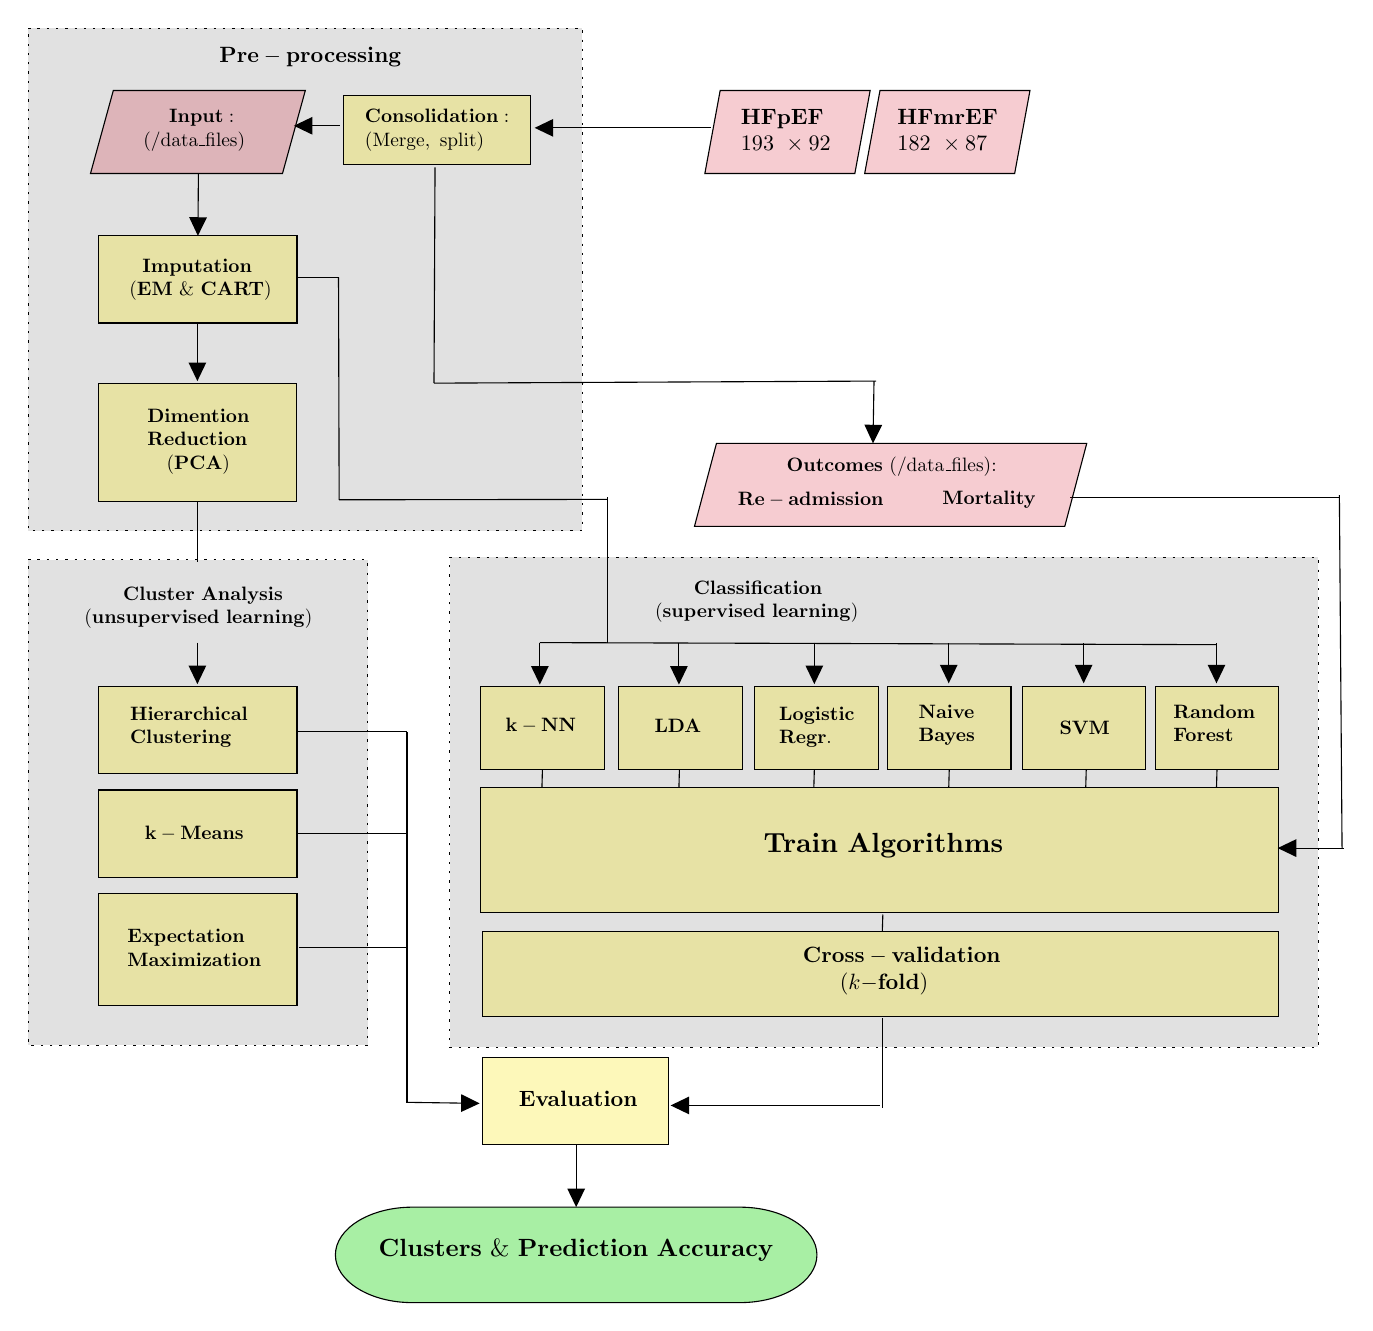
\begin{tikzpicture}[x=0.75pt,y=0.75pt,yscale=-1,xscale=1]
%uncomment if require: \path (0,646); %set diagram left start at 0, and has height of 646

%Shape: Rectangle [id:dp17767432122865645] 
\draw  [fill={rgb, 255:red, 155; green, 155; blue, 155 }  ,fill opacity=0.3 ][dash pattern={on 0.84pt off 2.51pt}] (2,5) -- (269,5) -- (269,247) -- (2,247) -- cycle ;
%Shape: Rectangle [id:dp17276791081063103] 
\draw  [fill={rgb, 255:red, 155; green, 155; blue, 155 }  ,fill opacity=0.3 ][dash pattern={on 0.84pt off 2.51pt}] (205,260) -- (623.5,260) -- (623.5,496) -- (205,496) -- cycle ;
%Shape: Rectangle [id:dp137712763597037] 
\draw  [fill={rgb, 255:red, 155; green, 155; blue, 155 }  ,fill opacity=0.3 ][dash pattern={on 0.84pt off 2.51pt}] (2,261) -- (165.5,261) -- (165.5,495) -- (2,495) -- cycle ;
%Straight Lines [id:da9350378875346577] 
\draw    (84,75) -- (83.77,103) ;
\draw [shift={(83.75,105)}, rotate = 270.48] [fill={rgb, 255:red, 0; green, 0; blue, 0 }  ][line width=0.75]  [draw opacity=0] (8.93,-4.29) -- (0,0) -- (8.93,4.29) -- cycle    ;

%Straight Lines [id:da9986924600189169] 
\draw    (83.5,147) -- (83.5,173) ;
\draw [shift={(83.5,175)}, rotate = 270] [fill={rgb, 255:red, 0; green, 0; blue, 0 }  ][line width=0.75]  [draw opacity=0] (8.93,-4.29) -- (0,0) -- (8.93,4.29) -- cycle    ;

%Straight Lines [id:da9104422198905568] 
\draw    (184.5,344) -- (184.5,523) ;


%Straight Lines [id:da17863107757037655] 
\draw    (184.5,522.5) -- (217.5,522.97) ;
\draw [shift={(219.5,523)}, rotate = 180.82] [fill={rgb, 255:red, 0; green, 0; blue, 0 }  ][line width=0.75]  [draw opacity=0] (8.93,-4.29) -- (0,0) -- (8.93,4.29) -- cycle    ;

%Straight Lines [id:da4423537570819638] 
\draw    (248.5,301) -- (248.5,319.22) ;
\draw [shift={(248.5,321.22)}, rotate = 270] [fill={rgb, 255:red, 0; green, 0; blue, 0 }  ][line width=0.75]  [draw opacity=0] (8.93,-4.29) -- (0,0) -- (8.93,4.29) -- cycle    ;

%Straight Lines [id:da14828368689404448] 
\draw    (315.5,301) -- (315.5,319.22) ;
\draw [shift={(315.5,321.22)}, rotate = 270] [fill={rgb, 255:red, 0; green, 0; blue, 0 }  ][line width=0.75]  [draw opacity=0] (8.93,-4.29) -- (0,0) -- (8.93,4.29) -- cycle    ;

%Straight Lines [id:da2745541849199835] 
\draw    (380.75,301) -- (380.75,319) ;
\draw [shift={(380.75,321)}, rotate = 270] [fill={rgb, 255:red, 0; green, 0; blue, 0 }  ][line width=0.75]  [draw opacity=0] (8.93,-4.29) -- (0,0) -- (8.93,4.29) -- cycle    ;

%Straight Lines [id:da10622223865111557] 
\draw    (445.5,301.39) -- (445.5,318.61) ;
\draw [shift={(445.5,320.61)}, rotate = 270] [fill={rgb, 255:red, 0; green, 0; blue, 0 }  ][line width=0.75]  [draw opacity=0] (8.93,-4.29) -- (0,0) -- (8.93,4.29) -- cycle    ;

%Straight Lines [id:da12728372488873485] 
\draw    (248.5,301) -- (574.5,302) ;


%Straight Lines [id:da04201945911359806] 
\draw    (413.5,482) -- (413.5,525) ;


%Straight Lines [id:da8309940078541183] 
\draw    (313.5,524) -- (412.5,524) ;

\draw [shift={(311.5,524)}, rotate = 0] [fill={rgb, 255:red, 0; green, 0; blue, 0 }  ][line width=0.75]  [draw opacity=0] (8.93,-4.29) -- (0,0) -- (8.93,4.29) -- cycle    ;
%Shape: Rectangle [id:dp805733141303524] 
\draw  [fill={rgb, 255:red, 248; green, 231; blue, 28 }  ,fill opacity=0.3 ] (220,371) -- (604.5,371) -- (604.5,431) -- (220,431) -- cycle ;
%Straight Lines [id:da5772744105119383] 
\draw    (281,231) -- (281,301) ;


%Straight Lines [id:da5307166780329797] 
\draw    (504,231) -- (634,231) ;


%Straight Lines [id:da8350224251535634] 
\draw    (633.71,230) -- (635,400) ;


%Shape: Rectangle [id:dp7689144799085996] 
\draw  [fill={rgb, 255:red, 248; green, 231; blue, 28 }  ,fill opacity=0.3 ] (36,105) -- (131.5,105) -- (131.5,147) -- (36,147) -- cycle ;
%Shape: Rectangle [id:dp8360402522569712] 
\draw  [fill={rgb, 255:red, 248; green, 231; blue, 28 }  ,fill opacity=0.3 ] (35.75,176) -- (131.25,176) -- (131.25,233) -- (35.75,233) -- cycle ;
%Shape: Rectangle [id:dp8436521642341313] 
\draw  [fill={rgb, 255:red, 248; green, 231; blue, 28 }  ,fill opacity=0.3 ] (36,322) -- (131.5,322) -- (131.5,364) -- (36,364) -- cycle ;
%Shape: Rectangle [id:dp8779924325569846] 
\draw  [fill={rgb, 255:red, 248; green, 231; blue, 28 }  ,fill opacity=0.3 ] (36,372) -- (131.5,372) -- (131.5,414) -- (36,414) -- cycle ;
%Shape: Rectangle [id:dp8944427225779763] 
\draw  [fill={rgb, 255:red, 248; green, 231; blue, 28 }  ,fill opacity=0.3 ] (36,422) -- (131.5,422) -- (131.5,476) -- (36,476) -- cycle ;
%Straight Lines [id:da12044404667160191] 
\draw    (131.5,344) -- (184.5,344) ;


%Straight Lines [id:da6084938483975053] 
\draw    (131.5,393) -- (184.5,393) ;


%Straight Lines [id:da16731103541967607] 
\draw    (132.5,448) -- (184.5,448) ;


%Straight Lines [id:da9753125405011336] 
\draw    (151.8,232.2) -- (281,232) ;


%Straight Lines [id:da8528567916678871] 
\draw    (151.5,125) -- (151.8,232.2) ;


%Straight Lines [id:da9889731806347037] 
\draw    (131.5,125) -- (151.5,125) ;


%Shape: Rectangle [id:dp8708975358842101] 
\draw  [fill={rgb, 255:red, 248; green, 231; blue, 28 }  ,fill opacity=0.3 ] (220,322) -- (279.5,322) -- (279.5,362) -- (220,362) -- cycle ;
%Shape: Rectangle [id:dp2832466894461272] 
\draw  [fill={rgb, 255:red, 248; green, 231; blue, 28 }  ,fill opacity=0.3 ] (286.5,322) -- (346,322) -- (346,362) -- (286.5,362) -- cycle ;
%Shape: Rectangle [id:dp14049594498977225] 
\draw  [fill={rgb, 255:red, 248; green, 231; blue, 28 }  ,fill opacity=0.3 ] (352,322) -- (411.5,322) -- (411.5,362) -- (352,362) -- cycle ;
%Shape: Rectangle [id:dp4503091833898072] 
\draw  [fill={rgb, 255:red, 248; green, 231; blue, 28 }  ,fill opacity=0.3 ] (416,322) -- (475.5,322) -- (475.5,362) -- (416,362) -- cycle ;
%Straight Lines [id:da37279512049375874] 
\draw    (249.5,371) -- (249.75,362) ;


%Straight Lines [id:da7877038245504153] 
\draw    (315.5,371) -- (315.75,362) ;


%Straight Lines [id:da47196717706905766] 
\draw    (380.5,371) -- (380.75,362) ;


%Straight Lines [id:da6265135418883228] 
\draw    (445.5,371) -- (445.75,362) ;


%Shape: Rectangle [id:dp23123927252195697] 
\draw  [fill={rgb, 255:red, 248; green, 231; blue, 28 }  ,fill opacity=0.3 ] (221,440) -- (604.5,440) -- (604.5,481) -- (221,481) -- cycle ;
%Straight Lines [id:da6647772541294572] 
\draw    (83.5,233) -- (83.5,262) ;


%Straight Lines [id:da7585523119166355] 
\draw    (413.5,440) -- (413.75,432) ;


%Straight Lines [id:da49016539083231736] 
\draw    (266,543) -- (266,571) ;
\draw [shift={(266,573)}, rotate = 270] [fill={rgb, 255:red, 0; green, 0; blue, 0 }  ][line width=0.75]  [draw opacity=0] (8.93,-4.29) -- (0,0) -- (8.93,4.29) -- cycle    ;

%Shape: Parallelogram [id:dp518581715076881] 
\draw  [fill={rgb, 255:red, 208; green, 2; blue, 27 }  ,fill opacity=0.2 ] (335.38,35) -- (407.64,35) -- (400.26,75) -- (328,75) -- cycle ;
%Straight Lines [id:da992949141941001] 
\draw    (83.5,301) -- (83.5,319) ;
\draw [shift={(83.5,321)}, rotate = 270] [fill={rgb, 255:red, 0; green, 0; blue, 0 }  ][line width=0.75]  [draw opacity=0] (8.93,-4.29) -- (0,0) -- (8.93,4.29) -- cycle    ;

%Straight Lines [id:da6160084227975695] 
\draw    (197.5,176) -- (410.5,175) ;


%Straight Lines [id:da3499925619434392] 
\draw    (409.5,175) -- (409.03,203) ;
\draw [shift={(409,205)}, rotate = 270.95] [fill={rgb, 255:red, 0; green, 0; blue, 0 }  ][line width=0.75]  [draw opacity=0] (8.93,-4.29) -- (0,0) -- (8.93,4.29) -- cycle    ;

%Straight Lines [id:da2578176252932385] 
\draw    (197.5,176) -- (198,72) ;


%Straight Lines [id:da924957907848829] 
\draw    (132,52) -- (152,52) ;

\draw [shift={(130,52)}, rotate = 0] [fill={rgb, 255:red, 0; green, 0; blue, 0 }  ][line width=0.75]  [draw opacity=0] (8.93,-4.29) -- (0,0) -- (8.93,4.29) -- cycle    ;
%Straight Lines [id:da09848220518746698] 
\draw    (248,53) -- (331,53) ;

\draw [shift={(246,53)}, rotate = 0] [fill={rgb, 255:red, 0; green, 0; blue, 0 }  ][line width=0.75]  [draw opacity=0] (8.93,-4.29) -- (0,0) -- (8.93,4.29) -- cycle    ;
%Shape: Parallelogram [id:dp8152627621795523] 
\draw  [fill={rgb, 255:red, 208; green, 2; blue, 27 }  ,fill opacity=0.2 ] (43,35) -- (135.5,35) -- (124.5,75) -- (32,75) -- cycle ;
%Shape: Parallelogram [id:dp9253495901859852] 
\draw  [fill={rgb, 255:red, 208; green, 2; blue, 27 }  ,fill opacity=0.2 ] (333.6,205) -- (512,205) -- (501.4,245) -- (323,245) -- cycle ;
%Shape: Parallelogram [id:dp42719482691252253] 
\draw  [fill={rgb, 255:red, 208; green, 2; blue, 27 }  ,fill opacity=0.2 ] (412.38,35) -- (484.64,35) -- (477.26,75) -- (405,75) -- cycle ;
%Flowchart: Terminator [id:dp16568399978235138] 
\draw  [fill={rgb, 255:red, 139; green, 233; blue, 134 }  ,fill opacity=0.75 ] (187.12,573) -- (344.88,573) .. controls (365.38,573) and (382,583.3) .. (382,596) .. controls (382,608.7) and (365.38,619) .. (344.88,619) -- (187.12,619) .. controls (166.62,619) and (150,608.7) .. (150,596) .. controls (150,583.3) and (166.62,573) .. (187.12,573) -- cycle ;
%Shape: Rectangle [id:dp14038294286941833] 
\draw  [fill={rgb, 255:red, 248; green, 231; blue, 28 }  ,fill opacity=0.3 ] (481,322) -- (540.5,322) -- (540.5,362) -- (481,362) -- cycle ;
%Shape: Rectangle [id:dp6127776736638881] 
\draw  [fill={rgb, 255:red, 248; green, 231; blue, 28 }  ,fill opacity=0.3 ] (545,322) -- (604.5,322) -- (604.5,362) -- (545,362) -- cycle ;
%Straight Lines [id:da7980328233946519] 
\draw    (510.5,301.39) -- (510.5,318.61) ;
\draw [shift={(510.5,320.61)}, rotate = 270] [fill={rgb, 255:red, 0; green, 0; blue, 0 }  ][line width=0.75]  [draw opacity=0] (8.93,-4.29) -- (0,0) -- (8.93,4.29) -- cycle    ;

%Straight Lines [id:da9962982021314886] 
\draw    (574.5,301.39) -- (574.5,318.61) ;
\draw [shift={(574.5,320.61)}, rotate = 270] [fill={rgb, 255:red, 0; green, 0; blue, 0 }  ][line width=0.75]  [draw opacity=0] (8.93,-4.29) -- (0,0) -- (8.93,4.29) -- cycle    ;

%Straight Lines [id:da5853970926877519] 
\draw    (606,400) -- (636,400) ;

\draw [shift={(604,400)}, rotate = 0] [fill={rgb, 255:red, 0; green, 0; blue, 0 }  ][line width=0.75]  [draw opacity=0] (8.93,-4.29) -- (0,0) -- (8.93,4.29) -- cycle    ;
%Shape: Rectangle [id:dp4763571703387559] 
\draw  [fill={rgb, 255:red, 248; green, 231; blue, 28 }  ,fill opacity=0.3 ] (221,501) -- (310.5,501) -- (310.5,543) -- (221,543) -- cycle ;
%Straight Lines [id:da7427067516231873] 
\draw    (511.5,371) -- (511.75,362) ;


%Straight Lines [id:da7011387804104916] 
\draw    (574.5,371) -- (574.75,362) ;



% Text Node
\draw (82,54) node [scale=0.7]  {$ \begin{array}{l}
\ \ \ \ \mathbf{Input:}\\
( /\mathrm{data\_files})
\end{array}$};
% Text Node
\draw (85,126) node [scale=0.7]  {$ \begin{array}{l}
\ \ \mathbf{Imputation}\\
\mathbf{( EM\ \&\ CART)}
\end{array}$};
% Text Node
\draw (84,204) node [scale=0.7]  {$ \begin{array}{l}
\mathbf{Dimention}\\
\mathbf{Reduction}\\
\ \ \ \mathbf{( PCA)}
\end{array}$};
% Text Node
\draw (81,342) node [scale=0.7]  {$ \begin{array}{l}
\mathbf{Hierarchical\ }\\
\mathbf{Clustering}
\end{array}$};
% Text Node
\draw (82,393) node [scale=0.7]  {$\mathbf{k-Means}$};
% Text Node
\draw (82,449) node [scale=0.7]  {$ \begin{array}{l}
\mathbf{Expectation}\\
\mathbf{Maximization}
\end{array}$};
% Text Node
\draw (84,284) node [scale=0.7]  {$ \begin{array}{l}
\ \ \ \ \ \ \mathbf{Cluster\ Analysis}\\
\mathbf{( unsupervised\ learning)}
\end{array}$};
% Text Node
\draw (249,341) node [scale=0.7]  {$\mathbf{k-NN}$};
% Text Node
\draw (315,341) node [scale=0.7]  {$\mathbf{LDA}$};
% Text Node
\draw (382,342) node [scale=0.7]  {$ \begin{array}{l}
\mathbf{Logistic}\\
\mathbf{Regr} .
\end{array}$};
% Text Node
\draw (446,341) node [scale=0.7]  {$ \begin{array}{l}
\mathbf{Naive\ }\\
\mathbf{Bayes}
\end{array}$};
% Text Node
\draw (414,459) node [scale=0.8]  {$ \begin{array}{l}
\ \ \ \ \ \mathbf{Cross-validation}\\
\ \ \ \ \ \ \ \ \ \ \mathbf{(} k\mathbf{-fold)}
\end{array}$};
% Text Node
\draw (353,281) node [scale=0.7]  {$ \begin{array}{l}
\ \ \ \ \ \ \mathbf{Classification}\\
\mathbf{( supervised\ learning)}
\end{array}$};
% Text Node
\draw (414,399) node   {$\mathbf{Train\ Algorithms}$};
% Text Node
\draw (266,594) node [scale=0.9]  {$\mathbf{Clusters\ \&\ Prediction\ Accuracy}$};
% Text Node
\draw (379,232) node [scale=0.7]  {$\mathbf{Re-admission}$};
% Text Node
\draw (465,232) node [scale=0.7]  {$\mathbf{Mortality}$};
% Text Node
\draw (418,216) node [scale=0.7]  {$\mathbf{Outcomes\ (} /\mathrm{data\_files})\mathbf{:}$};
% Text Node
\draw (445,55) node [scale=0.8]  {$ \begin{array}{l}
\mathbf{HFmrEF}\\
182\ \times 87
\end{array}$};
% Text Node
\draw (367,55) node [scale=0.8]  {$ \begin{array}{l}
\mathbf{HFpEF}\\
193\ \times 92
\end{array}$};
% Text Node
\draw  [fill={rgb, 255:red, 248; green, 231; blue, 28 }  ,fill opacity=0.3 ]  (154,37.5) -- (244,37.5) -- (244,70.5) -- (154,70.5) -- cycle  ;
\draw (199,54) node [scale=0.7]  {$ \begin{array}{l}
\mathbf{Consolidation} :\\
(\mathrm{Merge,\ split})
\end{array}$};
% Text Node
\draw (138,19) node [scale=0.8]  {$\mathbf{Pre-processing}$};
% Text Node
\draw (511,342) node [scale=0.7]  {$\mathbf{SVM}$};
% Text Node
\draw (575,341) node [scale=0.7]  {$ \begin{array}{l}
\mathbf{Random\ }\\
\mathbf{Forest}
\end{array}$};
% Text Node
\draw (267,521) node [scale=0.8]  {$\mathbf{Evaluation}$};

\end{tikzpicture}

\caption[Machine learning procedure adopted in the thesis]{\textit{Machine learning procedure adopted in the thesis}}
\label{fig:ML_proc_thesis}
\normalsize
\end{figure}

\indent The machine learning procedure adopted in this thesis is illustrated in Figure (\ref{fig:ML_proc_thesis}). The procedure starts by pre-processing the data. This pre-processing step consists of three sub processes: consolidation, imputation and dimension reduction. The consolidation process merges the HFpEF and HFmrEF datasets into one data set with the same types of variables. In addition to having one data set with all the observations, the process also leaves the data separate (but with equal variables), so that an analysis on each separate data set can be done. Furthermore, the clinical outcomes of the patients in the data set are extracted by this process and stored for later use in the classification part of the thesis. The imputation process imputes missing data to ensure that the data is balanced, and the dimensional reduction process (principal component analysis (PCA)) addresses eventual problems with higher dimensional multi-correlated variables. The pre-processing step is explained in further detail later in this chapter (see section \ref{sec:data}). After the pre-processing is done, the procedure continues by first addressing the cluster analysis. We use the principal components derived from the dimension reduction process as input into the clustering algorithms evaluated. The cluster analysis runs the produced components through the three cluster algorithms (hierarchical clustering, k-means and expectation maximization). After the procedure is done, three sets of clusters are produced. The next step is to evaluate the clusters by assessing their level of homogeneity. This is done by comparing the number of significantly different baseline characteristics.\\
\indent The supervised classification track is structured in a somewhat different way. The imputed data is run through the six classification algorithms (k-NN, LR, NB, LDA, SVM and RF). The data is trained with principal component analysis and validated with 10-fold cross-validation to produce approximately unbiased estimates of the test errors/accuracy. The accuracy are also adjusted by means of the Cohens' Kappa $\kappa$. After the data is run thought the classification process and the accuracy is calculated, the algorithms are ranked and evaluated accordingly. The outputs of the whole ML procedure are i) clinical clusters that \textit{may} have distinct phenotypical properties and ii) the accuracy of the various classification algorithms in predicting readmission and mortality in the data sets. All the processes mentioned in the ML procedure in Figure (\ref{fig:ML_proc_thesis}) are developed using the \texttt{R} statistical programming language (version 3.4.4 - \textit{Someone to Lean On}) \citep{Rsoftware2018} with RStudio as the integrated development environment (IDE), version 1.1.423 \citep{RStudio2018}. We use a number of external libraries and self-made algorithms in order to make the whole research process more efficient. Data description with variable explanations, descriptive statistics and some relevant plots can be found in appendix (\ref{chap:data_desc}). The source code used to produce all the results in this thesis, can also be found in appendix (\ref{chap:souce_code}). As we now have given an overview of the ML procedure used in this thesis, we move on to presenting the data.

\section{Data}
\label{sec:data}

\noindent The data used is comprised of two data sets (\texttt{data\_use\_HFpEF.mat}, dim: $193 \times 92$ and \texttt{data\_use\_HFmrEF.mat}, dim: $182 \times 87$). Since both data sets have different types of clinical variables, we consolidated the data into three main data sets with the same number and types of variables: 
\begin{enumerate}[label=(\roman*)]
    \item Full sample (\texttt{HFfullDataSet.Rdat}, dim: $374 \times 55$)
    \item HFpEF sample (\texttt{HFpEFdataSet .Rdat}, dim: $193 \times 55$)
    \item HFmrEF sample (\texttt{HFmrEFdataSet.Rdat}, dim: $182 \times 55$)
\end{enumerate}
\indent The data was collected by the medical staff at a tertiary hospital in the United Kingdom. At this particular hospital NT-proBNP led heart failure service were run on all patients with suspected heart failure. All patients with suspected HF based on an assessment of the HF probability and raised NT-proBNP/BNP levels (see Figure \ref{fig:esc_algo_hf}) were included and forwarded for an echocardiography. An expert HF physician reviewed all the patients after the echocardiography was performed. The patients were diagnosed with HF according to the 2016 ESC guidelines \citep{ponikowski2016}. Accordingly, signs and symptoms of HF, raised NP values, echocardiographic results including left ventricular ejection fraction (LVEF) and evidence of structural or functional heart abnormalities were the primary basis for the assessment done by the hospitals cardiac physicians. After the diagnosis, patients were categorized based on LVEF following the ESC guidelines, i.e. patients with LVEF $>$ 50\% were classified as HFpEF and those with $40 \leq$ LVEF $< 50$ as HFmrEF. The patients with LVEF $<$ 40\%, greater than moderate valvular heart disease and prior cardiac transplantation were excluded. The data was collected over a one-year period from October 10th 2014 to October 9th 2015. In total 375 patients were analyzed over this one-year period with data from almost 100 clinical features being recorded. The outcomes were evaluated through the hospital databases and mortality was confirmed with the Office for National Statistics. All the data was collected as part of the hospitals approved Clinical Audit. As mentioned in the previous section, we reduced the SL problem in the supervised learning part of the ML procedure to a two-class classification problem. The way this was done was with respect to the various \texttt{patient\_groups} in the data. The patients were grouped based on various \noindent outcomes. In total six outcome categories were  defined in the data sets. The outcome categories are as follows: \texttt{IN} - inhospital mortality, \texttt{Z} \noindent mortality within 30 days, \texttt{Y} - mortality within 1 year, \texttt{X} - mortality by Fluorouracil (medication), \texttt{V} - cardiac readmission within 30 days, \texttt{U} - readmission and \texttt{R} - the rest. The various combinations of the outcome classes found in the data sets, and the way in which they were classified, are listed in Table (\ref{tab:outcomes_class}). From this table, we can\\



\begin{footnotesize}
\begin{tabularx}{\textwidth}{LLLLLLLLLLL}
\caption{Clinical outcome classes}\label{tab:outcomes_class}\\
\toprule
\multicolumn{10}{c}{PANEL I: Full Sample (\texttt{HFfullDataSet.Rdat})}\\
\midrule
\multicolumn{2}{l}{\textbf{Group}} & \multicolumn{2}{l}{Dead?} & \multicolumn{2}{l}{Readm?} & \multicolumn{2}{l}{$n$} & \multicolumn{2}{l}{\% Tot}\\ 
\midrule
\multicolumn{2}{l}{R} &    \multicolumn{2}{l}{no}  & \multicolumn{2}{l}{no} &  \multicolumn{2}{l}{186} & \multicolumn{2}{l}{0.496} \\ 
\multicolumn{2}{l}{U} &    \multicolumn{2}{l}{no}  & \multicolumn{2}{l}{yes} & \multicolumn{2}{l}{59} &  \multicolumn{2}{l}{0.157} \\ 
\multicolumn{2}{l}{X, R} & \multicolumn{2}{l}{yes} & \multicolumn{2}{l}{no} &  \multicolumn{2}{l}{29} &  \multicolumn{2}{l}{0.077} \\ 
\multicolumn{2}{l}{Y} &    \multicolumn{2}{l}{yes} & \multicolumn{2}{l}{no} &  \multicolumn{2}{l}{16} &  \multicolumn{2}{l}{0.043} \\ 
\multicolumn{2}{l}{IN} &   \multicolumn{2}{l}{yes} & \multicolumn{2}{l}{no} &  \multicolumn{2}{l}{15} &  \multicolumn{2}{l}{0.040}\\ 
\multicolumn{2}{l}{V} &    \multicolumn{2}{l}{no}  & \multicolumn{2}{l}{yes} & \multicolumn{2}{l}{15} &  \multicolumn{2}{l}{0.040}\\ 
\multicolumn{2}{l}{Y, U} & \multicolumn{2}{l}{yes} & \multicolumn{2}{l}{yes} & \multicolumn{2}{l}{13} &  \multicolumn{2}{l}{0.035} \\ 
\multicolumn{2}{l}{X, U} & \multicolumn{2}{l}{yes} & \multicolumn{2}{l}{yes} & \multicolumn{2}{l}{11} &  \multicolumn{2}{l}{0.029} \\ 
\multicolumn{2}{l}{Y, V} & \multicolumn{2}{l}{yes} & \multicolumn{2}{l}{yes} & \multicolumn{2}{l}{11} &  \multicolumn{2}{l}{0.029} \\ 
\multicolumn{2}{l}{X} &    \multicolumn{2}{l}{yes} & \multicolumn{2}{l}{no} &  \multicolumn{2}{l}{9 }&   \multicolumn{2}{l}{0.024} \\ 
\multicolumn{2}{l}{Z} &    \multicolumn{2}{l}{yes} & \multicolumn{2}{l}{no} &  \multicolumn{2}{l}{7 }&   \multicolumn{2}{l}{0.019} \\ 
\multicolumn{2}{l}{X, V} & \multicolumn{2}{l}{yes} & \multicolumn{2}{l}{yes} & \multicolumn{2}{l}{3 }&   \multicolumn{2}{l}{0.008} \\ 
\multicolumn{2}{l}{Z, V} & \multicolumn{2}{l}{yes} & \multicolumn{2}{l}{yes} & \multicolumn{2}{l}{1 }&   \multicolumn{2}{l}{0.003} \\ 
\midrule
\multicolumn{10}{c}{PANEL II: Outcome Classes by Clinical Syndrome}\\
\midrule
\multicolumn{5}{c}{HFpEF (\texttt{HFpEFdataSet.Rdat})} & \multicolumn{5}{c}{HFmrEF (\texttt{HFmrEFdataSet.Rdat})}\\
\midrule
\textbf{Group} & Dead? & Readm? & $n$ & \% Tot & \textbf{Group} & Dead? & Readm? & $n$ & \% Tot \\ 
\midrule
R & no & no & 85 & 0.440 & R & no & no & 101 & 0.555 \\ 
U & no & yes & 40 & 0.207 & U & no & yes & 19 & 0.104 \\ 
X, R & yes & no & 29 & 0.150 & Y & yes & no & 15 & 0.082 \\ 
V & no & yes & 10 & 0.052 & IN & yes & no & 8 & 0.044 \\ 
IN & yes & no & 7 & 0.036 & X & yes & no & 8 & 0.044 \\ 
Y, U & yes & yes & 7 & 0.036 & Z & yes & no & 7 & 0.038 \\ 
Y, V & yes & yes & 7 & 0.036 & Y, U & yes & yes & 6 & 0.033 \\ 
X, U & yes & yes & 6 & 0.031 & V & no & yes & 5 & 0.027 \\ 
X & yes & no & 1 & 0.005 & X, U & yes & yes & 5 & 0.027 \\ 
Y & yes & no & 1 & 0.005 & Y, V & yes & yes & 4 & 0.022 \\ 
&  &  &  &  & X, V & yes & yes & 3 & 0.016 \\ 
&  &  &  &  & Z, V & yes & yes & 1 & 0.005 \\
\midrule
\end{tabularx}
\end{footnotesize}

\vspace*{-0,5cm}\noindent  see that approximately 36.8\% of all the patients in the HFpEF data set were readmitted in some form, i.e either within 30 days or more. In the HFmrEF data set, this number was somewhat smaller being approximately 23.4\%. In the full sample, approximately 29.1\% of the patients were readmitted. The number also differed with respect to whether the patients were confirmed deceased or not. In the HFpEF data set, approximately 29.9\% of the patients had confirmed mortality and in the HFmrEF data set this number was 31.1\%. For the full sample, the number is approximately 30.7\%. Further descriptive statistics on the data can be found in appendix (\ref{sec:desc_stat}). The source code for the two-class outcome classification shown in Table (\ref{tab:outcomes_class}), can be found in appendix (\ref{sec:app_desc_stat}). As the data used in this thesis is cross-sectional, we need to emphasize that it is not ideal. Limitations to the data sets are many and one of the most relevant one is that of missing data. 

\subsection{Missing data}
\label{subsec:miss_data}

\noindent Missing values in data is a very important concept in data management and a highly prevalent problem in any data analysis. If one does not handle missing values properly, this may lead to inaccurate or invalid inference being drawn from the data. Results where improper treatment of missing data is present may differ significantly from those where missing data is  



\begin{footnotesize}
\begin{tabularx}{\textwidth}{P{2.3cm}LLLLP{2.7cm}LLLL}
\caption{Summary of missing values}\label{tab:top_missing}\\
\toprule
\multicolumn{10}{c}{PANEL I: Full Sample (\texttt{HFfullDataSet.Rdat})}\\
\midrule
\multicolumn{2}{l}{\textbf{Variable (V)}}& \multicolumn{2}{l}{\#Na} & \multicolumn{2}{l}{\%$n$} & \multicolumn{2}{l}{\%Na} & \multicolumn{2}{l}{\%V} \\ 
\midrule
\multicolumn{2}{l}{grand.tot      } & \multicolumn{2}{l}{3081}  & \multicolumn{2}{l}{0.149} & \multicolumn{2}{l}{1.000} & \multicolumn{2}{l}{     } \\ 
\midrule
\multicolumn{2}{l}{irondef        } & \multicolumn{2}{l}{254 }  & \multicolumn{2}{l}{0.012} & \multicolumn{2}{l}{0.082} & \multicolumn{2}{l}{0.677} \\ 
\multicolumn{2}{l}{ferritin       } & \multicolumn{2}{l}{250 }  & \multicolumn{2}{l}{0.012} & \multicolumn{2}{l}{0.081} & \multicolumn{2}{l}{0.667} \\ 
\multicolumn{2}{l}{bmiadmission   } & \multicolumn{2}{l}{223 }  & \multicolumn{2}{l}{0.011} & \multicolumn{2}{l}{0.072} & \multicolumn{2}{l}{0.595} \\ 
\multicolumn{2}{l}{ironlevels     } & \multicolumn{2}{l}{210 }  & \multicolumn{2}{l}{0.010} & \multicolumn{2}{l}{0.068} & \multicolumn{2}{l}{0.560} \\ 
\multicolumn{2}{l}{tsat           } & \multicolumn{2}{l}{210 }  & \multicolumn{2}{l}{0.010} & \multicolumn{2}{l}{0.068} & \multicolumn{2}{l}{0.560} \\ 
\multicolumn{2}{l}{timetohfadm    } & \multicolumn{2}{l}{184 }  & \multicolumn{2}{l}{0.009} & \multicolumn{2}{l}{0.060} & \multicolumn{2}{l}{0.491} \\ 
\multicolumn{2}{l}{pasp           } & \multicolumn{2}{l}{181 }  & \multicolumn{2}{l}{0.009} & \multicolumn{2}{l}{0.059} & \multicolumn{2}{l}{0.483} \\ 
\multicolumn{2}{l}{admissionwgt   } & \multicolumn{2}{l}{164 }  & \multicolumn{2}{l}{0.008} & \multicolumn{2}{l}{0.053} & \multicolumn{2}{l}{0.437} \\ 
\multicolumn{2}{l}{ecgqrsduration } & \multicolumn{2}{l}{141 }  & \multicolumn{2}{l}{0.007} & \multicolumn{2}{l}{0.046} & \multicolumn{2}{l}{0.376} \\ 
\multicolumn{2}{l}{obesity        } & \multicolumn{2}{l}{137 }  & \multicolumn{2}{l}{0.007} & \multicolumn{2}{l}{0.044} & \multicolumn{2}{l}{0.365} \\ 
\midrule
\multicolumn{5}{c}{HFpEF (\texttt{HFpEFdataSet.Rdat})} & \multicolumn{5}{c}{HFmrEF (\texttt{HFmrEFdataSet.Rdat})}\\
\midrule
\textbf{Variable (V)}& \#Na & \%$n$ & \%Na & \%V & \textbf{Variable (V)} & \#Na & \%$n$ & \%Na & \%V \\ 
\midrule
grand.tot &         973 & 0.092 & 1 &  & grand.tot & 2108 & 0.211 & 1 &  \\ 
\midrule
irondef & 124 & 0.012 & 0.127 & 0.642 & bmiadmission & 178 & 0.018 & 0.084 & 0.978 \\ 
timetohfadm & 124 & 0.012 & 0.127 & 0.642 & admissionwgt & 131 & 0.013 & 0.062 & 0.720 \\ 
ferritin & 122 & 0.011 & 0.125 & 0.632 & irondef & 130 & 0.013 & 0.062 & 0.714 \\ 
tsat & 99 & 0.009 & 0.102 & 0.513 & obesity & 129 & 0.013 & 0.061 & 0.709 \\ 
ironlevels & 98 & 0.009 & 0.101 & 0.508 & ferritin & 128 & 0.013 & 0.061 & 0.703 \\ 
pasp & 71 & 0.007 & 0.073 & 0.368 & breathless & 127 & 0.013 & 0.060 & 0.698 \\ 
bmiadmission & 45 & 0.004 & 0.046 & 0.233 & ironlevels & 112 & 0.011 & 0.053 & 0.615 \\ 
ee & 41 & 0.004 & 0.042 & 0.212 & tsat & 111 & 0.011 & 0.053 & 0.610 \\ 
ecgqrsduration & 36 & 0.003 & 0.037 & 0.187 & pasp & 110 & 0.011 & 0.052 & 0.604 \\ 
ecgrate & 34 & 0.003 & 0.035 & 0.176 & ecgqrsduration & 105 & 0.010 & 0.050 & 0.577 \\
\midrule
\end{tabularx}
\end{footnotesize}

\noindent not present. In medical research, it is not uncommon for patient data to be missing. Missing data from patients clinical variables are typically defined as the values that are not directly observed \citep{ibrahim2012missing}. Data can be missing due to a number of reasons. In clinical research some reasons may include: poor communication with study subject, difficulties assessing the clinical outcomes, lack of consolidation from test, duration of trial etc. The latter is often a reason for missing data, as longer trials tend to produce more risk of missing data. Especially considering that patients often run the risk of being dropped from the studies before completion \citep{myers2000handling}. In our data sets, the problem with missing values is very much present. In the full data set, a total of 3081 observations are missing accounting for about 14.9\% of the total data set. The main non-indicator variables accounting for the highest amount of this number is the lack of registering ferritin levels (\texttt{ferritin}, 8.1\% of missing), BMI at admission (\texttt{bmiadmission}, 7.2\%), ironlevels (\texttt{ironlevels}, 6.8\%), transferrin saturation (\texttt{tsat}, 6.8\%), time of HF admission (\texttt{timetohfadm}, 6\%), pulmonary artery systolic pressure (\texttt{pasp}, 5.9\%), weight at admission (\texttt{admissionwgt}, 5.3\%) and ECQ QRS duration (\texttt{ecgqrsduration}, 4.6\%). We can also look at the missing values in both sub data sets. In the HFpEF data set a total of 973 observations, i.e. approximately 9.2\% of the data set is missing. Of the non-indicator variables, the largest contributors can be attributed to the failure of registering time to HF admission (\texttt{timetohfadm}, 12.7\% of missing), ferritin levels (\texttt{ferritin}, 12.5\%), transferrin saturation (\texttt{tsat}, 10.2\%), iron levels (\texttt{ironlevels}, 10.1\%), pulmonary artery systolic pressure (\texttt{pasp}, 7.3\%), registering body-mass-index (BMI) at admission (\texttt{bmiadmission}, 4.6\%), E/e' ratio (\texttt{ee}, 4.2\%), ECQ QRS duration (\texttt{ecgqrsduration}, \texttt{3.7\%}) and ECG rate (\texttt{ecgrate}, 3.5\%). These variables contribute to approximately 68.8\% of the missing values in the HFpEF data. In the HFmrEF data set, the picture is very much different. In general, we can say that this data set has a much larger presence of missing values even though the clinical variables used in both sets are the same. In total 2108 observations, i.e. approximately 21.1\% of the data is missing. The largest non-indicator contributors are: inability to record the body mass index (BMI) at admission (\texttt{bmiadmission}, 8.4\%), the weight of patients at admission (\texttt{admissionwgt}, 6.2\%), ferritin levels (\texttt{ferritin}, 6.1\%), iron levels (\texttt{ironlevels}, 5.3\%), transferrin saturation (\texttt{tsat}, 5.3\%), pulmonary artery systolic pressure (\texttt{pasp}, 5.2\%) and ECQ QRS duration (\texttt{ecgqrsduration}, \texttt{5\%}). These variables account for 41.1\% of the missing values in the HFmrEF data. An overview of the variables with the most missing values in each data set can be found in Table (\ref{tab:top_missing}).

\subsection{Little's test for MCAR}
\label{subsec:little}

\noindent The presence of missing values has to be addressed by any individual conducting data analysis. Missing values may make the data corrupted and introduce statistical bias that may lead to invalid results and inferences. This is vital for us as many of the statistical methods used later in this thesis cannot be conducted in the presence of missing values. When talking about missing values one typically mention three distinct types of missing values, see e.g. \cite{sterne2009multiple} and \cite{kaushal2014missing} for further explanation. These are as follows:

\begin{enumerate}[label=(\roman*)]
    \item Missing completely at random (MCAR): This type assumes that there is no systematic difference between the missing values and the observed values. An example can be if blood pressure values are missing due to breakdown in automatic sphygmomanometer, or if blood sugar values are missing due to a non working glucometer.
    \item Missing at random (MAR): The second type of missing values assumes that any difference between the missing values and the observed values can be explained by differences in the observed values. Again, an example can be that missing blood pressure values or blood sugar values may be lower than the measured values, but only because younger people may be more likely to have missing blood pressure and blood sugar as missing.
    \item Missing not at random (MNAR): The last and final type assumes that even after the observer data are taken into account, the systematic differences between the observed and missing values are still present. An example can be that people with high values of blood pressure or blood sugar may be less likely to attend an appointment due to headache.  
\end{enumerate}

\noindent MNAR can only be speculated and thus never determined, see e.g. \cite{rubin1976inference}, \cite{schafer2002missing} and \cite{moons2006using}. In our data, we assume that the missing data is at least missing at random (MAR). This is an assumption that many in the literature place on their data without any attempt at supplying some arguments to support such an assumption. To this we have carried out Little's MCAR test \citep{little1988test} on our data (separately on indicator and continuous variables). The test is structured with the following three steps : 
\begin{enumerate}[label=(\roman*)]
    \item The test starts by using the expectation-maximization (EM) algorithm \citep{dempster1977maximum} to estimate the maximum likelihood of the population mean $\bm{\tilde{\mu}}_{obs, j}$ and variance-covariance matrix $\bm{\tilde{\Sigma}}_{obs,j}$. Here one enters the $Y:N\times p$ matrix of data into the EM algorithm.
    \item Next step is to create a set of matrices $S_j$ for $j = 1, \hdots, J$ where each matrix of the data set consists of all cases that are identified with particular missing patterns (0 = not-missing and 1 = missing). Define $m_j$ to be the number of cases that belong to a given missing response pattern in $S_j$. From these $J-1$ cases, calculate the \textit{observed} vector of means $\bm{\hat{y}}_{obs, j}$ for each random response pattern. 
    \item The final step comprises of calculating the difference between the observed means in step 2 with the estimated EM-means from step 1 weighted by $m_j$ and the inverse variance-covariance matrix to obtain the following test statistics:
    \begin{align}
        d^2 = \sum_{j=1}^J m_j \left(\bm{\hat{y}}_{obs, j} -  \bm{\tilde{\mu}}_{obs, j}\right)\bm{\tilde{\Sigma}}_{obs,j}^{-1}\left(\bm{\hat{y}}_{obs, j} -  \bm{\tilde{\mu}}_{obs, j}\right)^T
    \end{align}
\end{enumerate}

\noindent \cite{little1988test} showed that $d^2$ is asymptotically $\chi^2$-distributed with $f = \sum_{j=1}^J p_j - p$ degrees of freedom, where $p_j$ is the number of observed variables for cases in $S_j$. Thus, with the use of $d^2$, a large-sample test of the MCAR assumption compares $d^2$ with a chi-squared distribution with $f$ df can be done, and rejecting the null hypothesis when $d^2$ is large. Following this procedure, we have carried out Little's MCAR test and the results are presented in Table (\ref{tab:little_test}). The results were produced using the function \texttt{LittleMCAR()} in the \texttt{r} package \texttt{BaylorEdPsych} \citep{BaylorEdPsych}. We removed the variables that had more than 15\% missing values from the


\begin{footnotesize}
\begin{tabularx}{\textwidth}{Lrrrrr}
\caption{Little's MCAR test}\label{tab:little_test}\\
\toprule
& num col & missing.patterns & Chi.squared ($\chi^2$) & df & $p$-value\\
\midrule
\endfirsthead
\caption*{\textbf{Table \ref{tab:little_test}:} Little's MCAR test (\textit{continued})}\\
\toprule
& num col & missing.patterns & Chi.squared ($\chi^2$) & df & $p$-value\\
\midrule
\endhead
\multicolumn{6}{c}{Panel I: HFpEF}\\
\midrule
indicator & 43 & 37 & 692.8908 & 662 & 0.19645 \\ 
continuous\_1 & 16 & 58 & 534.3060 & 542 & 0.58493 \\ 
continuous\_2 & 16 & 83 & 720.2238 & 751 & 0.78464 \\ 
continuous\_3 & 17 & 49 & 330.3824 & 383 & 0.97567 \\
\midrule
\multicolumn{6}{c}{Panel II: HFmrEF}\\
\midrule
indicator.1 & 49 & 135 & 2331.4367 & 2276 & 0.20470 \\ 
continuous\_1.1 & 15 & 71 & 409.6785 & 440 & 0.84708 \\ 
continuous\_2.1 & 15 & 19 & 106.9243 & 105 & 0.42938 \\
\midrule
\end{tabularx}
\end{footnotesize} 

\noindent HFpEF data set, 25\% from the HFmrEF data set and 20\% from the full data set (see table \ref{tab:top_missing} for top 10 missing variables). Next, we split the variables into two data sets, one for the continuous variables and one for the indicator variables. We also removed the variables that had near zero variance using the \texttt{nearZeroVar()} function in the \texttt{caret} package \citep{kuhncaret}. As remarked by \cite{BaylorEdPsych}, the \texttt{LittleMCAR()} function can be very time inefficient for data sets with more than 50 variables. This time inefficiency is why we split the data sets into the two subsets, i.e. continuous and indicator and thus conducted separate tests on both subsets. The test assumes that the data is MCAR, and this is accordingly the null-hypothesis. From Table (\ref{tab:little_test}), we can see that all the $p$-values are insignificant at 5\% significance level. This suggests that we cannot reject the null hypothesis of the missing data  
\noindent being MCAR. However, as argued by \cite{allison1999missing}, just because the data passes this test, does not mean that the MCAR assumption is satisfied. The assumptions for MCAR are strong, and a simple test such as the one suggested by \cite{little1988test} does not in and of itself satisfy those assumptions. It merely lends evidence in its support, and given the test results presented in Table (\ref{tab:little_test}), we consider this assumption to be intact. When it comes to the question regarding missing values, there exists many ways of dealing with this problem. Each of these ways have different advantages as well as disadvantages. One of the most common way of dealing with missing values is through the use of imputation techniques. This is something we will present in the next section.

\vspace*{-0,5cm}\subsection{Imputation}
\label{subsec:impu}

\noindent There exists a wide variety of methods that fall under the class of imputation. In general, all methods that attempt to replace each missing value in a data set with an estimate or a guess, are typically classified as being an imputation method \citep{allison1999missing}. A very popular and conventional method of imputing missing values is through the use of mean imputation. This method implies swapping each missing value with the mean of the observed values in the given variable column. The method is very easy to use and maintains the sample size, but it has a problem with underestimating both the variance and standard deviation estimates. This implies that the estimates that produce the imputed values are unbiased see e.g. \cite{scheffer2002dealing}, \cite{enders2010applied} and \cite{eekhout2012brief}. Another class of imputation method that have proven to handle missing values in a wide variety of cases, is the maximum likelihood methods. The use of set methods requires that the assumption of MCAR is intact and if this is done, can produce estimates that have the desirable properties normally associated with maximum likelihood. These properties are consistency (estimates will be approximately unbiased in large samples), asymptotic efficiency (estimates are close to being fully efficient i.e., having minimal standard errors) and asymptotic normality (allows the use of normal approximation to calculate confidence intervals and $p$-values). Additionally, the use of maximum likelihood methods can produce standard errors that fully account for the fact that some data is missing \citep{allison1999missing}. It is exactly based on these qualities that we have chosen maximum likelihood based imputation as one of the strategies to address the problem with the missing values in our data set presented in subsection (\ref{subsec:miss_data}). We have also shown that this is relevant as the assumption of MCAR is assumed intact, see subsection (\ref{subsec:little}).\\
\indent A maximum likelihood method typically starts out by expressing a likelihood function. This function expresses the probability of the data as a function of the unknown parameters. Assuming two discrete random variables: $\mathbf{X}$ and $\mathbf{Z}$ with a joint probability function defined by $p(x,z|\boldsymbol{\theta})$, where $\boldsymbol{\theta}$ is a vector of parameters. The joint probability function gives us the probability that $\mathbf{X} = x$ and $\mathbf{Z} = z$. If we assume no missing values and that the observations are independent, i.e. $cov(\mathbf{X}, \mathbf{Z}) = 0$, then the likelihood function is defined by:
\begin{align}
    L(\boldsymbol{\theta}) = \prod_{i=1}^n p(x_i, z_i | \boldsymbol{\theta})
    \label{eq:likelihood}
\end{align}
\noindent To find an estimate of the maximum likelihood, we need to find the value for $\boldsymbol{\theta}$ that maximizes the likelihood function (eq. \ref{eq:likelihood}). This can be done using the log-likelihood function ($\mathcal{L} (\boldsymbol{\theta}) = \log L(\boldsymbol{\theta})$) and should give us an estimate defined by:
\begin{align}
    {\displaystyle {\hat {\theta }}\in \left \{{\underset {\theta \in \Theta }{\operatorname {arg\,max} }}\ \sum_{i=1}^n\log p (x_i, z_i | \boldsymbol{\theta})\right \}}
\end{align}
\noindent If we assume that the data is MAR on $\boldsymbol{Z}$ for the first $r$ cases, and MAR on $\boldsymbol{X}$ for the next $s$ cases, we can then split the likelihood function into parts that correspond to each missing value pattern and accordingly factor these parts. This is in order to get a likelihood function that takes into account the missing data patterns. The likelihood function becomes as follows:
\begin{align}
    L(\boldsymbol{\theta}) = \prod_{i=1}^r g(x_i | \boldsymbol{\theta})\prod_{i=r+1}^{r+s} h(z_i | \boldsymbol{\theta})\prod_{i=r+s+1}^n p(x_i, z_i | \boldsymbol{\theta}) 
\end{align}
\noindent where $g(x | \theta)$ and $h(z | \theta)$ are the marginal distributions of $\boldsymbol{X}$ and $\boldsymbol{Z}$, so that:
\begin{align}
    \prod_{i = 1}^r g(x_i | \boldsymbol{\theta}) \prod_{i = r + 1}^{r + s} h(z_i | \boldsymbol{\theta}) = \prod_{i=1}^{r+s} p(x_i, z_i | \boldsymbol{\theta})
\end{align}
\noindent For each missing data pattern, the likelihood is found by summing the joint distribution over all possible values of the variables with missing data. The estimated maximum likelihood parameters in this particular example should therefore be defined by:
\begin{align}
    {\displaystyle {\hat {\theta }}\in \left \{{\underset {\theta \in \Theta }{\operatorname {arg\,max} }}\ \left(\sum_{i=1}^{r+s}\log p(x_i, z_i | \boldsymbol{\theta}) + \sum_{i=r+s+1}^n\log p (x_i, z_i | \boldsymbol{\theta})\right)  \right\}}
\end{align}
\noindent We assumed the variables were discrete in the begin, and as such if the variables were continuous, the summations would be replaced by integrals. The extension to multiple variables is also relatively straightforward \citep{allison1999missing}. In order to implement a maximum likelihood method on data that contains missing values, it is important to have a model for the joint distribution for all variables in the data set, and accordingly have a numerical method for maximizing the likelihood of this distribution. Determining this model can vary with the type of data that one is dealing with.\\
\indent In our data set, we have both continuous and indicator variables. When the data is continuous it is common to assume a multivariate-normal model, i.e. that all the variables are independently identically normally distributed (iid) and can be expressed as a linear function of all other variables (or subsets). There is also an assumption that the errors are homoscedastic, i.e. constant and have a mean of 0. In the case of the indicator variables, it is difficult to assume that these variables are normally distributed. However, according to \cite{schafer1997analysis}, \cite{schafer1998multiple} and \cite{allison1999missing} simulation evidence and practical experience have shown that maximum likelihood methods can do a good job in imputing missing values, even if the variables in question are indicator variables. Still, we opted to use a different imputation method for each of the types of data, i.e. we use a bootstrapped expectation-maximization (EM) imputation method for the variables that are continuous and a classification- and regression tree (CART) based imputation method for the indicator variables.\\
\indent As we mentioned, one needs to have a numerical method for maximizing the likelihood of the joint probability distribution. One of the most common numerical methods is the expectation-maximization (EM) algorithm \citep{dempster1977maximum}. We mentioned it slightly in subsection (\ref{subsec:little}), but it is an iterative algorithm that is used to maximize the likelihood function (eq. \ref{eq:likelihood}) of a number of missing data models. It is comprised of two steps; the expectation step (often called the $E$ step) and the maximization step (called the $M$ step). In the expectation step, the expected values of the log-likelihood is taken over the variables with missing values using the current estimated parameters \citep{allison1999missing}. Afterwards the maximization step involves maximizing the expected log-likelihood in order to get new estimates of the parameters. These two steps are continued until convergence is achieved, i.e. until the estimated parameters of the joint probability distribution doesn't change from one iteration to the next. Most standard software packages using an EM implementation have as a principal output a set of maximum likelihood parameters related to the joint probability distribution. The imputed values are often included in addition, but are not recommended for further analysis. The reason for this is that these imputed values are not designed for that purpose and as such will produce biased estimates of many parameters if used in further analysis \citep{allison1999missing}.\\
\indent A way to get around this problem is using multiple-imputation. \cite{honaker2011amelia}  introduced a bootstrapped EM algorithm that combines the nice properties of the EM algorithm, i.e. consistency, asymptotic efficiency etc. with the accuracy property of the bootstrap re-sampling method, see \cite{efron1992bootstrap} and \cite{james2013introduction}. \cite{honaker2011amelia} also argue that the EMB algorithm they developed is much faster and more reliable than alternative algorithms, in addition to making valid and much more accurate imputations for cross-sectional data. The algorithm is implemented in the \texttt{Amalie II} package in \texttt{r}. The assumptions of the algorithm are as follows: if we assume that the data set can be expressed as a matrix $\boldsymbol{D}$ consisting of dimensions $(n\times k)$. Let the matrix $\boldsymbol{D}$ be comprised of two parts, i.e. $\boldsymbol{D^{mis}}$ the missing part and $\boldsymbol{D^{obs}}$ the observer part. The matrix $\boldsymbol{D}$ is assumed to follow a multivariate distribution with mean vector $\boldsymbol{\mu}$ and covariance matrix $\boldsymbol{\Sigma}$. This assumption can be stated as $\boldsymbol{D} \sim N\left(\boldsymbol{\mu},  \boldsymbol{\Sigma}\right)$. In addition to the multivariate normality assumption, the algorithm assumes that the data is MAR. The latter have we already shown to be intact, but the first assumption is somewhat difficult. As the data is by definition incomplete due to the missing data, we assume that this assumption is intact. Typically one would test if this assumption is intact by using a multivariate normality test similar to the ones mentioned by \cite{mardia1970measures}, \cite{henze1990class} or \cite{royston1982extension}. Most of these tests assume that the data is complete, and should the data be incomplete then it is common to remove the missing observations and conduct the tests on the remaining data. The challenge for our part is that approximately 15\% of our data set is missing which may cast doubt on the statistical power that these tests may have. As a result of this, we have chosen to assume that the normality assumption is intact. The schematic approach of this algorithm and the way it used in this thesis is described in Figure (\ref{fig:BEM_algo}). The procedure starts by producing $n$ bootstrapped data sets for which the EM algorithm is run on each bootstrapped data sets.  For all the data sets in the thesis, i.e. the full data (\texttt{HFfullDataSet.Rdat}), HFmrEF (\texttt{HFmrEFdataSet.Rdat}) and HFpEF \texttt{HFpEFdataSet.Rdat} we let the algorithm produce $n = 100$ bootstrapped data sets. After the imputed data sets are produced they are collapsed by averaging all the imputed values produced by the EM algorithm. All the data from the incomplete data set that the procedure started with should be the same, with the exception of the missing values, i.e. these have been replaced by the average of the imputed values.

\begin{figure}

\centering





\tikzset{every picture/.style={line width=0.75pt}} %set default line width to 0.75pt        

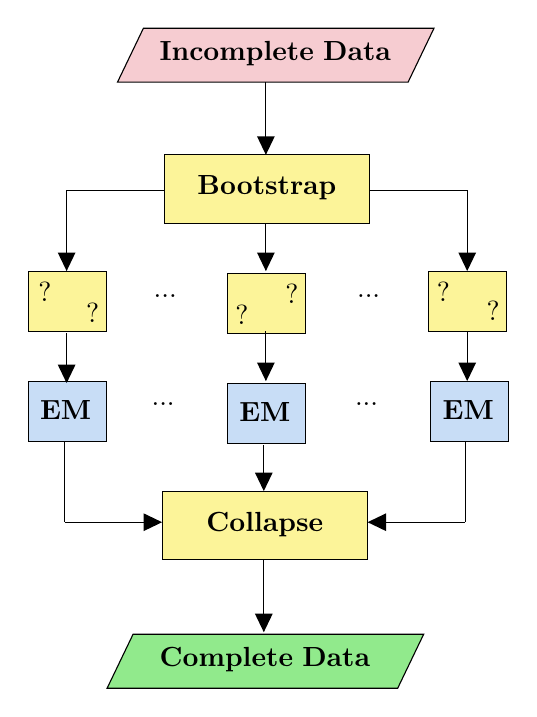
\begin{tikzpicture}[x=0.75pt,y=0.75pt,yscale=-1,xscale=1]
%uncomment if require: \path (0,652); %set diagram left start at 0, and has height of 652

\draw  [fill={rgb, 255:red, 208; green, 2; blue, 27 }  ,fill opacity=0.2 ] (244.5,3) -- (384.5,3) -- (372,29) -- (232,29) -- cycle ;
\draw    (303.5,29) -- (303.5,62) ;
\draw [shift={(303.5,64)}, rotate = 270] [fill={rgb, 255:red, 0; green, 0; blue, 0 }  ][line width=0.75]  [draw opacity=0] (8.93,-4.29) -- (0,0) -- (8.93,4.29) -- cycle    ;

\draw  [fill={rgb, 255:red, 248; green, 231; blue, 28 }  ,fill opacity=0.45 ] (254.5,64) -- (353.5,64) -- (353.5,97) -- (254.5,97) -- cycle ;
\draw    (207.5,81) -- (254.5,81) ;


\draw    (353.5,81) -- (400.5,81) ;


\draw    (207.5,81) -- (207.5,118) ;
\draw [shift={(207.5,120)}, rotate = 270] [fill={rgb, 255:red, 0; green, 0; blue, 0 }  ][line width=0.75]  [draw opacity=0] (8.93,-4.29) -- (0,0) -- (8.93,4.29) -- cycle    ;

\draw    (400.5,81) -- (400.5,118) ;
\draw [shift={(400.5,120)}, rotate = 270] [fill={rgb, 255:red, 0; green, 0; blue, 0 }  ][line width=0.75]  [draw opacity=0] (8.93,-4.29) -- (0,0) -- (8.93,4.29) -- cycle    ;

\draw    (303.5,97) -- (303.5,118) ;
\draw [shift={(303.5,120)}, rotate = 270] [fill={rgb, 255:red, 0; green, 0; blue, 0 }  ][line width=0.75]  [draw opacity=0] (8.93,-4.29) -- (0,0) -- (8.93,4.29) -- cycle    ;

\draw  [fill={rgb, 255:red, 248; green, 231; blue, 28 }  ,fill opacity=0.45 ]  (189, 120) rectangle (226.5, 149)   ;
\draw  [fill={rgb, 255:red, 248; green, 231; blue, 28 }  ,fill opacity=0.45 ]  (285, 121) rectangle (322.5, 150)   ;
\draw  [fill={rgb, 255:red, 248; green, 231; blue, 28 }  ,fill opacity=0.45 ]  (382, 120) rectangle (419.5, 149)   ;
\draw    (207.5,150) -- (207.5,172) ;
\draw [shift={(207.5,174)}, rotate = 270] [fill={rgb, 255:red, 0; green, 0; blue, 0 }  ][line width=0.75]  [draw opacity=0] (8.93,-4.29) -- (0,0) -- (8.93,4.29) -- cycle    ;

\draw    (303.5,149) -- (303.5,171) ;
\draw [shift={(303.5,173)}, rotate = 270] [fill={rgb, 255:red, 0; green, 0; blue, 0 }  ][line width=0.75]  [draw opacity=0] (8.93,-4.29) -- (0,0) -- (8.93,4.29) -- cycle    ;

\draw    (400.5,149) -- (400.5,171) ;
\draw [shift={(400.5,173)}, rotate = 270] [fill={rgb, 255:red, 0; green, 0; blue, 0 }  ][line width=0.75]  [draw opacity=0] (8.93,-4.29) -- (0,0) -- (8.93,4.29) -- cycle    ;

\draw  [fill={rgb, 255:red, 74; green, 144; blue, 226 }  ,fill opacity=0.3 ]  (189, 173) rectangle (226.5, 202)   ;
\draw  [fill={rgb, 255:red, 74; green, 144; blue, 226 }  ,fill opacity=0.3 ]  (285, 174) rectangle (322.5, 203)   ;
\draw  [fill={rgb, 255:red, 74; green, 144; blue, 226 }  ,fill opacity=0.3 ]  (383, 173) rectangle (420.5, 202)   ;
\draw    (206.5,202) -- (206.5,241) ;


\draw    (399.5,202) -- (399.5,241) ;


\draw    (302.5,204) -- (302.5,224) ;
\draw [shift={(302.5,226)}, rotate = 270] [fill={rgb, 255:red, 0; green, 0; blue, 0 }  ][line width=0.75]  [draw opacity=0] (8.93,-4.29) -- (0,0) -- (8.93,4.29) -- cycle    ;

\draw    (206.5,241) -- (251.5,241) ;
\draw [shift={(253.5,241)}, rotate = 180] [fill={rgb, 255:red, 0; green, 0; blue, 0 }  ][line width=0.75]  [draw opacity=0] (8.93,-4.29) -- (0,0) -- (8.93,4.29) -- cycle    ;

\draw    (354.5,241) -- (399.5,241) ;

\draw [shift={(352.5,241)}, rotate = 0] [fill={rgb, 255:red, 0; green, 0; blue, 0 }  ][line width=0.75]  [draw opacity=0] (8.93,-4.29) -- (0,0) -- (8.93,4.29) -- cycle    ;
\draw  [fill={rgb, 255:red, 248; green, 231; blue, 28 }  ,fill opacity=0.45 ] (253.5,226) -- (352.5,226) -- (352.5,259) -- (253.5,259) -- cycle ;
\draw    (302.5,259) -- (302.5,292) ;
\draw [shift={(302.5,294)}, rotate = 270] [fill={rgb, 255:red, 0; green, 0; blue, 0 }  ][line width=0.75]  [draw opacity=0] (8.93,-4.29) -- (0,0) -- (8.93,4.29) -- cycle    ;

\draw  [fill={rgb, 255:red, 139; green, 233; blue, 134 }  ,fill opacity=0.95 ] (239.5,295) -- (379.5,295) -- (367,321) -- (227,321) -- cycle ;

\draw (308,15) node   {$\mathbf{Incomplete\ Data}$};
\draw (304,80) node   {$\mathbf{Bootstrap}$};
\draw (197,130) node  [align=left] {?};
\draw (220,140) node  [align=left] {?};
\draw (292,141) node  [align=left] {?};
\draw (316,131) node  [align=left] {?};
\draw (389,130) node  [align=left] {?};
\draw (413,139) node  [align=left] {?};
\draw (207,187) node   {$\mathbf{EM}$};
\draw (303,188) node   {$\mathbf{EM}$};
\draw (401,187) node   {$\mathbf{EM}$};
\draw (303,242) node   {$\mathbf{Collapse}$};
\draw (303,307) node   {$\mathbf{Complete\ Data}$};
\draw (255,132) node   {$...$};
\draw (353,132) node   {$...$};
\draw (254,184) node   {$...$};
\draw (352,184) node   {$...$};


\end{tikzpicture}

\caption[BEM procedure]{\textit{Bootstrapped Expectation Maximization (BEM) procedure}}
\label{fig:BEM_algo}

\end{figure}

\indent For the indicator variables, the imputation technique is defined by a classification- and regression tree (CART) algorithm. This algorithm is implemented in the \texttt{mice} package in \texttt{r} \citep{buuren2010mice}. The implementation proceeds as follows: for each variable $\boldsymbol{k}$ in the matrix $\boldsymbol{D}$, the algorithm fits a classification or regression three by recursive partitioning. Then for each missing value in $\boldsymbol{k}$, the algorithm finds the terminal nodes, i.e. the nodes the missing value can end up in according to the fitted tree. Lastly, the algorithm makes a random draw among the members in the nodes, and takes the observed value from that draw as the imputation. Rather than collapsing the multiple imputed data sets as with the BEM algorithm, we simply use the first imputed data sets for further analysis. Further description of the procedure of the algorithm can be found in \cite{burgette2010multiple}. Our implementation of the algorithms with the source code can be found in appendix (\ref{sec:utilities}). This concludes our treatment of the challenge with missing data in this thesis. Next, we present our treatment of the challenge with the higher dimensional data in the thesis.

\subsection{Dimensional reduction}
\label{subsec:dim_red}

\noindent As we can see from Figure (\ref{fig:ML_proc_thesis}), the number of features in each HF data sets are 92 and 87. After the consolidation process, we reduce the number of features to 39 in each data sets. The problem with higher dimensional data is that some of these features may be noise features that are not truly associated with a given response. This may lead to a deterioration in a fitted model, and thus increase the uncertainty. Noise features may also exacerbate the risk of overfitting, i.e. having a statistical model that contains more parameters than can be justified by the data \citep{friedman2009elements}, \citep{james2013introduction}. One can also run the risk of drawing invalid inference, as many of the features may be correlated with each other and thus one may face the case of multicollinearity, i.e. risking inflated standard errors.\\
\indent We have chosen to address this problem with the use of Principal Component Analysis (PCA). The purpose of PCA is to express the information in the data set $\mathbf{D}$ by a lower number of variables $\mathbf{Z}$, called principal components. These principal components act as a lower dimensional representation of the data that contains as much as possible of the variation in the original dataset. Each of the principal components are computed as linear combinations of the $p$ features, and are orthogonal and linearly uncorrelated. This property is ideal for addressing the challenge with multicollinearity.\\
\indent For a given $n \times p$ data set $\mathbf{D}$, we assume that each of the variables has been centered to have mean zero. We then want the linear combination of the sample feature values of the form $z_{i1} = \theta_{11}x_{i1} + \theta_{21}x_{i2} + \hdots + \theta_{p1}x_{ip}$ that has the largest sample variance, subject to the constraint $\sum_{j = 1}^p \theta_{j1}^2 = 1$. The optimization problem becomes \citep{james2013introduction}:
\begin{align}
    \max_{\theta_{11}, \hdots, \theta_{p1}} \left\{\frac{1}{n} \sum_{i=1}^n \left(\sum_{j=1}^p \theta_{j1}x_{ij} \right)^2 \right\} \hspace{0,25cm} \text{subject to} \hspace{0,25cm} \sum_{j=1}^p\theta^2_{j1} = 1
\end{align}
\noindent In the optimization problem above, we want to maximize the sample variance of the $n$ values of $z_{i1}$. The elements $z_{11}, \hdots ,z_{n1}$ are referred to as the \textit{scores} of the first component, and solving the optimization problem can be done using an eigen value decomposition. One can compute these principal components by using the estimated correlation or co-variance matrix of $\mathbf{D}$. We have chosen to use the correlation matrix and the implementation of this is done using the \texttt{princomp()} function in the \texttt{stats}-package in \texttt{r}, \citep{stats}. We run the imputed data sets produced in subsection (\ref{subsec:impu}) through the PCA function and select the first principal components that explain most of the variance in the data set for further analysis. The number of components used for the full sample data set is 4, which explains approximately 27\% of the variation in the original data set. For the other data sets, i.e. the HFpEF and HFmrEF datasets, we use the first two principal components. These explain approximately 15\% of the variation in the orginal data set. In the succeeding analysis, we use these principal components as input to the cluster analysis. Much of the literature on the topic applies the same procedure to address the challenge of higher dimensional data, see e.g. \cite{shah2014phenomapping}, \cite{ahmad2014clinical} and \cite{katz2017phenomapping}. 

\section{Clustering patient groups}
\label{sec:cluster_pat_gro}

\noindent In this section, we present the unsupervised clustering algorithms used in this thesis. The clustering algorithms used are as mentioned: hierarchical, k-means and expectation-maximization (EM) clustering. As there exists many clustering algorithm, we follow the strategy defined in section (\ref{sec:overview}) and try to keep to the ones most used in the literature. An overview of the implementation and the source code can be found in appendix (\ref{sec:clust}).

\vspace*{-0,25cm}\subsection{Hierarchical}
\label{subsec:hierarchical}

\noindent The first clustering algorithm evaluated in the cluster analysis process is the hierarchical clustering algorithm, \cite{sibson1973slink}, \cite{defays1977efficient} and \citep{rohlf198212}. This algorithm uses a simple algorithm that takes into account the dissimilarity between clusters and accordingly produces a graphical representation in the form of a dendrogram. The algorithm starts by calculating\\

\begin{algorithm}[H]{
\SetAlgoLined
\textit{initialization}\;
\hspace*{0,5cm}$n$ observations\\
\hspace*{0,5cm}Distance measure\\
\hspace*{0,5cm}Treat every observation $n$ as its own cluster\\
    \For{$i = n, n-1, \hdots, 2$}{                    
        Examine and fuse the most similar clusters\\
        Compute the pairwise inter-cluster dissimilarities\\ \hspace*{0,5cm}among the $i - 1$ remaining clusters
    }
}
Cut dendrogram based on max relative loss of inertia criteria\\
\Return Clusters
\caption{Hierarchical clustering}
\end{algorithm}\vspace*{0,5cm}

\noindent the dissimilarity between each pairs of observations, i.e. the patients. A common measure of the dissimilarity is the euclidean distance between pairs of observations. For all clustering algorithms where the distance is required, we have assumed that the euclidean distance measure is the most optimal. However, there exists many other distance measures, e.g. squared, polynomial, Manhattan, maximum and Mahalanobis distance that may be equally optimal. After calculating the distance, the algorithm starts at the bottom of the dendrogram, i.e. where the observations are the most similar, and treats each of the $n$ observations as its own clusters. Next, the algorithm fuses the two clusters that are most similar and this continued iteratively for the remaining $n - 1$ clusters. When the algorithm is finished and the dendrogram is complete, all the clusters are now part of the same cluster. It is then up to the user to choose where to cut the dendrogram. In our implementation, we cut the dendrogram based on the criteria of maximizing the relative loss of inertia. The pseudocode for this algorithm is presented above.\\
\indent The advantage of the hierarchical clustering algorithm, is that one does not need to define the number of clusters a priori, and thus a user can cut the dendrogram at any given height based on a given index or heuristic. There are many implementations of this algorithm, but since we use the principal components as input to this and all the other clustering algorithms, we have chosen to use the Hierarchical Clustering on Principal Components function \texttt{HCPC()} in the \texttt{FactoMineR}-package in \texttt{r} \citep{FactoMineR}. We have also created our own function (\texttt{pca.var.plot()}) that visually presents the clustering results from all the clustering algorithms chosen for evaluation in this thesis. This function is very useful as it can supply the user with a visual illustration of the clustering results for each clustering algorithm. The evaluation criteria used to evaluate the clustering methods is something that we will be addressing in later sections. The hierarchical clustering algorithm is, however, just one of the algorithms that we use and accordingly, we now move on to explaining the k-means algorithm.

\vspace*{-0,25cm}\subsection{k-means}
\label{subsec:K-Means}

\noindent The k-means clustering algorithm \citep{forgy1965cluster} is a prototype-based technique for partitioning data into a pre-defined number of clusters ($K$). The clusters are represented by the centroids (means) of the clusters \citep{tan2007introduction}. The algorithm assumes that each observation $x_i$ belongs to at least one of the $K$ clusters and that the clusters are non-overlapping, i.e. that no observations belong to more than one cluster. The idea behind the k-means clustering algorithm is that a good clustering is one that minimizes the within-cluster variation, i.e. a measure of how much the amount of observations within a cluster varies $W(C_k)$, where $C_k$ is the set containing the indices of the observations in cluster $K$. Similar to the hierarchical clustering algorithm, this measure is often the euclidean distance between each pair of observations. Accordingly, the algorithm seeks to solve the following optimization problem \citep{james2013introduction}:

\begin{align}
    \min_{C_i, \cdots, C_k} \left\{\sum_{k=1}^K \frac{1}{|C_k|} \sum_{i,i^\star \in C_k}\sum_{j=1}^P\left(x_{ij} - x_{i^\star j} \right)^2 \right\}\hspace*{0,25cm}\text{where}\hspace*{0,25cm} i \neq i^\star
\end{align}

\noindent The solution to this optimization problem is very difficult as there exists $K^n$ possible ways of partitioning $n$ observations into $K$ clusters. The k-means algorithm solves this problem with the following steps represented with the following pseudocode:\\

\begin{algorithm}[H]{
\SetAlgoLined
\textit{initialization}\;
    \hspace*{0,5cm}$n$ observations\\
    \hspace*{0,5cm}Distance measure\\
    \hspace*{0,5cm}The number of clusters $K$ to be produced\\
   \For{$i = 1, \hdots, n$}{                    
        Randomly assign a number in $\left \{1, K \right \}$ to $i$
    }
    \While{Cluster assignment continuous to change}{
        \For{Each cluster $C_k$}{
            Compute cluster centroid\\
            \For{Each observation in $C_k$}{
                Assign each observation to the cluster\\ \hspace*{0,5cm}whose centroid is closest
            }
        }    
    }
    \Return Clusters
}
\caption{k-means clustering}
\end{algorithm}\vspace*{0,5cm}

\noindent The algorithm takes as input $n$ observations, the defined distance measure and the number of clusters $K$ to be produced. Then all the observations $n$ are assigned a number in the set of the number corresponding to the clusters. This assignment is done at random and serves as the initial cluster assignment for the observations. Then the algorithm iterates until there is no change in cluster assignment between cluster assignment $a_t$ and $a_{t-1}$. The cluster assignments is done by computing the cluster centroid and assigning each observation in the cluster $C$ to the cluster $C_1, \hdots, C_k$ whose centroid is closest, i.e. given the distance measure. \\
\indent The disadvantage of the k-means algorithm is that it requires a user to define the number  of clusters a priori, which in some cases may be seen as defeating the purpose of the cluster analysis, i.e. the results may vary with the number of clusters chosen. We have tried to address this problem by using the \texttt{r} function \texttt{NbClust()} \citep{nbclust} that uses almost 25 indices for determining the number of clusters and proposes to the user the "optimal" number of clusters by the use of a majority-rule of all the indices. As for the actual implementation of the k-means clustering algorithm, we use the \texttt{kmeans()} function in the \text{stats}-package \citep{stats}. The implementation of this algorithm is wrapped in the \texttt{pca.cluster.plot()} function we mentioned in the preceding section.

\vspace*{-0,25cm}\subsection{Expectation-maximization}
\label{subsec:em}

\noindent The k-means algorithm is closely related to the EM algorithm \citep{dempster1977maximum} for estimating certain Gaussian mixture model(s). As we mentioned in section (\ref{subsec:impu}), the EM algorithm consists of estimating the maximum likelihood parameters of the given Gaussian(s) in question. This is done in the E-step of the algorithm and as such this is responsible for assigning the "responsibilities" for each data points based on its relative density under each mixture components. Whilst the M-step is responsible for recomputing the component density parameters based on the current responsibilities \citep{friedman2009elements}. The aim of the EM clustering algorithm is to assign the data into $K$ clusters according to the observations probability of belonging to each of the clusters. It is often stated that the EM algorithm is a "soft" version of the k-means algorithm, as the points are assigned based on a probabilistic (rather than a deterministic) approach \citep{james2013introduction}. The pseudocode for the EM algorithm is given below. Accordingly, the algorithm starts by having the user input the data matrix $\mathbf{D}$, a parametric model $f_\theta$, an initial distribution $\pi_0$ and a randomly selected parameter vector $\boldsymbol{\theta}$. The algorithm then computes the expected responsibilities of each observations and updates the parameters $\boldsymbol{\theta}$ with the maximum likelihood estimates $\boldsymbol{\theta}_{max}$. This is done iteratively until convergence. Being that the EM algorithm is similar to the k-means algorithm, it has also the same disadvantages, i.e. the user needs to define the number of clusters to be produced a priori. In addition, it can sometimes be very time consuming or even impossible for the algorithm to achieve convergence, i.e. no changes in cluster assignment between iterations. In theory, as the exit criteria of the EM algorithm may be defined by convergence, this could mean that the algorithm may never stop as convergence is not guaranteed in all cases. One could however define an exit criteria as a set number of iterations $i_{max}$ to terminate the algorithm, but this is something we have not done and accordingly the algorithm stops once convergence is reached. As for the implementation, we use the \texttt{Mclust()} function in the \texttt{mclust} package in \texttt{r} \citep{mclust}. All the default setting are used in the implementation and as with the previous clustering algorithms, the EM algorithm is also wrapped in the \texttt{pca.var.plot()} function.\\

\begin{algorithm}[H]{
\SetAlgoLined
\textit{initialization}\;
    \hspace*{0,5cm}Data set $\mathbf{D} = \left \{X_1, \hdots, X_n \right\}$\\
    \hspace*{0,5cm}Parametric model $f_\theta$\\
    \hspace*{0,5cm}Choose an initial distribution $\pi_0$ and pick\\ \hspace*{1cm}a parameter vector $\boldsymbol{\theta}$ at random.\\
    \While{No convergence}{
        \textbf{E step}:\\
        Compute expected responsibilities on each observation\\
        \textbf{M step}:\\
        Update the parameters in $\boldsymbol{\theta}$ with the likelihood\\
        \hspace*{0,5cm}maximization parameters $\boldsymbol{\theta}_{\max}$.
    }
    \Return Clusters produced by EM process
}
\caption{EM clustering}
\end{algorithm}

\vspace*{-0,25cm}\section{Classifying clinical outcomes}
\label{sec:classify_clin_out}

\noindent In this section, we present the supervised classification algorithms used in this thesis. As we mention in section (\ref{sec:overview}), the classification algorithms that will be evaluated are: k-nearest neighbours, logistic regression, naive Bayes, linear discriminant analysis, support vector machines and random forest. We will also mention the way in which we evaluate the algorithms with the K-fold cross validation. All the source code can be found in appendix (\ref{chap:souce_code}).

\subsection{k-nearest neighbours}
\label{subsec:knn}

\noindent The first algorithm we will be presenting is the k-nearest neighbours (k-NN) algorithm. The k-NN algorithm \citep{fix1951discriminatory} is a widely used algorithm, and often for good reason. It is very intuitive and simple to understand. In addition, the algorithm performs very well in many cases. This classifier is a memory-based algorithm that classifies a given observation based on the $k$ nearest neighbours of that observation in the feature space. Mathematically, given a query point $x_0$, the k-NN algorithm tries to find the $k$ training points $x_{(r)}, r = 1, \hdots, k$ closest in distance to $x_0$, and thus classify the point $x_0$ according to the majority rule of the $k$ closest points to $x_0$, see \citep{friedman2009elements} and \citep{james2013introduction}. The pseudocode for the algorithm is given below. Based on the pseudocode, we can see that the k-NN algorithm starts out by taking as input the training data $\mathbf{X}$ which is a subset of the full dataset ${\displaystyle \mathbf{X}\subseteq \mathbf{D}}$, the class labels $\mathbf{Y}$ of $\mathbf{X}$ and the distance measure to be used $d$. The distance measure between two data points are typically assumed to be a Minkowski distance:
\begin{align}
    d[i,j] = \left(\sum_{i=1}^n |X_{i, k} - X_{j, k}|^p\right)^{1/q}
\end{align}
where if $p=1$ or 2, the distance $d$ will correspond to the Manhattan or the Euclidean distance. As $q$ approaches infinity, the distance measure $d$ convergence to the maximum distance, i.e. the largest coordinate difference between data points. After computing the distance between data points, the algorithm classifies the labels of the unknown sample $x$ based on the mapping learned by the training data done with the majority rule.\\
\indent The observant reader will probably wonder how the unknown sample $x$ is determined. This is something we will address in a later section dealing with cross-validation. However, what we can say is that the implementation of the k-NN algorithm used in this thesis is that of the \texttt{knn()} function from the \texttt{stats} package in \texttt{r} \citep{stats}. We also need to emphasize that the k-NN algorithm is not without disadvantages. That is, the k-NN algorithm is slow when one has many observations, since it does not generalize over data in advance. It scans all the data each time a prediction is needed. It also has disadvantages with higher dimensional data as even normalizing the data makes the distances "blurred". This is because the distance to all neighbors becomes more or less the same in higher dimensional space. Another critique of the k-NN algorithm is that it in many ways classifies observations based on heuristics, i.e. it lacks probabilistic intuition and rational similar to other classification algorithms. Still, it is very popular and one that we will attempt to examine in this thesis.\\

\begin{algorithm}[H]{
\SetAlgoLined
\textit{initialization}\;
    \hspace{0.5cm} $\mathbf{X}$: training data\\
    \hspace{0.5cm} $\mathbf{Y}$: class labels of $\mathbf{X}$\\
    \hspace{0.5cm} $x$: unknown sample\\
    \hspace{0.5cm} Distance measure $d$\\
    \For{$i=1, \hdots, n$}{
        Compute distance $d(\mathbf{X}_i, x)$
    }
    Compute set $I$ containing indices for the $k$ smallest\\
    \hspace*{0,5cm}distances $d(\mathbf{X}_i, x)$.\\
    \Return Majority label for $\left\{ \mathbf{Y}_i \hspace{0.25cm} \text{where} \hspace{0.25cm} i \in I \right\}$
}
\caption{k-NN classification algorithm}
\end{algorithm}


\subsection{Logistic regression}
\label{subsec:logr}

\noindent Logistic regression is a very popular classification algorithm in medical research. The algorithm uses a logistic function to model the dependent discrete class labels corresponding to a given observation. In our example, the algorithm tries to model the probability that a given patient "belongs" to a particular clinical outcome (mortality or readmission) using a probabilistic approach. In the case of modeling this probability using multiple predictors, the algorithm tries to estimate the probability using the following generalized logistic function \citep{friedman2009elements}:
\begin{align}
    P(X) = \frac{\exp \left\{\beta_0 + \sum_{i=1}^p\beta_iX_i \right\}}{1 +\exp \left\{\beta_0 + \sum_{i=1}^p\beta_iX_i \right\}}
    \label{eq:logr}
\end{align}

\noindent Where $X = \left(X_1, \hdots, X_p \right)$ are the independent variables. The slope parameters $\beta_0, \hdots, \beta_p$ are estimated using the maximum likelihood, i.e. each slope parameter $\beta_i$ is estimated so that the following holds:

\begin{align}
    \hat{\beta} \in \left\{ {\underset {\beta \in \Theta }{\operatorname {arg\,max} }}\ \sum_{i=1}^p\log p(x_i, \beta)\right\}
\end{align}

\noindent Unlike linear regression, logistic regression uses the logistic function (\ref{eq:logr}) to map the patient to a given clinical outcome. The mapping is done by selecting a threshold $p^\star$ and if the calculated probability is above this threshold, we assign the given patient to that particular clinical outcome. In our case, we use $p^\star = 0.50$ as this is the default value in the implementation. Logistic regression works well for categorical outcomes, but has a significant disadvantage in working with response variables of continuous scale. The algorithm also requires that each data point be independent of all other data points. Should this not be the case, then the model may tend to overweight the significance of those observations, \cite{friedman2009elements} and \cite{james2013introduction}. Still, logistic regression is one of the most used algorithms in medical statistics. It is a relatively "simple" algorithm that perform very well in classification, see e.g. \cite{austin2013using} and \cite{zolfaghar2013big}. The implementation of this algorithm is done using the \texttt{glm()} function from the \texttt{stats}-package in \texttt{r} \citep{stats}. All default arguments are used with the exception of \texttt{family = binomial(link='logit')} which guarantees that the link function is the logistic function (eq. \ref{eq:logr}).

\subsection{Naive Bayes}
\label{subsec:nb}

\noindent The naive Bayes algorithm (also called "simple" Bayes) is a popular probabilistic classifier used to classify data based on the probability that a given observation belongs to a particular class. It is in many ways very similar to logistic regression, but the classifier is based on the Bayes theorem and assumes that the effect of an attribute value on a given class is independent of the value of the other attributes. For a given classification problem, we want to determine $P(H | \boldsymbol{X})$, i.e. the probability that the hypothesis \textit{H} holds given the "evidence" (i.e. the \textit{observed} data sample $\boldsymbol{X}$). The probability $P(H | \boldsymbol{X})$ is also known as the posteriori probability and is according to Bayes' theorem calculated by the following:
\begin{align}
    p(H | \boldsymbol{X}) = \frac{p(\boldsymbol{X}|H) p(H)}{p(\boldsymbol{X})} 
\end{align}
\noindent The probabilities $p(\boldsymbol{X}|H)$, $p(\boldsymbol{X})$ and $p(H)$ can all be estimated from the given data sample. The procedure for which the algorithm classifies a given observation into a discrete categorical outcome is given by the following \citep{leung2007naive}. Given a sample $\boldsymbol{X}$, the naive Bayes' classifier will predict that $\boldsymbol{X}$ belongs to the class having the highest posteriori probability, \textit{conditioned} on $\boldsymbol{X}$. That is $X$ is predicted to belong to the class $C_i$ if and only if $P(C_i| \boldsymbol{X}) > P(C_j | \boldsymbol{X})$ for $1 \leq j \leq n$, $j \neq i$. Rather than using a threshold value $p^\star$ as with logistic regression, one seeks to maximize the posteriori probability and accordingly assign labels to observations. For large sample data sets the naive Bayes' classifier is especially appropriate as it can outperform many sophisticated algorithms. However, the assumption of independence among the variables is often very unrealistic and although it simplifies the estimation, the risk of high bias is very much present with the algorithm. In this thesis we will be implementing the Naive Bayes algorithm using the \texttt{nb()} function in the \texttt{caret} package \citep{kuhncaret}.

\subsection{Linear discriminant analysis}
\label{subsec:lda}

\noindent The LDA algorithm is very similar to principal component analysis (PCA). Both try to look for linear combinations that best explain the data. However, LDA, tries explicitly to model the difference between the classes of data. This is done by modeling the distribution of the predictors $X$ separately in each of the response classes. The objective of LDA is to perform dimension reduction (similar to PCA), while preserving as much of the class discrimination information as possible. Assuming we have a $p$ dimensional random variable $X$, where $X$ follows a multivariate normal distribution, i.e. $X \sim N(\mu,\boldsymbol{\Sigma})$. This distribution is formally given by the following, see \cite{friedman2009elements} and \cite{james2013introduction}:
\begin{align}
    f(x) = \frac{1}{(2\pi)^{p / 2}|\boldsymbol{\Sigma}|^{1/2}} \exp\left \{-\frac{1}{2}(x-\mu)^T \boldsymbol{\Sigma}^{-1} (x - \mu) \right \}
    \label{seq:multi_normal}
\end{align}

\noindent In the case where we have $p > 1$ independent variables, the LDA classifier assumes that the observation in the $k$th class is drawn from a multivariate normal distribution $N(\mu_k, \boldsymbol{\Sigma})$. Plugging eq. (\ref{seq:multi_normal}) into the formula for the posterior probability and solving for the Bayes classifier yields:

\begin{align}
    \delta_k (x) = x^T\boldsymbol{\Sigma}^{-1} \mu_k - \frac{1}{2}\mu_k^T\boldsymbol{\Sigma}^{-1} \mu_k + \log \pi_k
    \label{eq:bayes_classifier}
\end{align}

\noindent Where $\pi_k$ is the prior probability that an observation belongs to the $k$th class. The LDA algorithm assigns a new observation $X=x$ by plugging the estimates of $\mu_1, \hdots, \mu_K, \pi_1, \hdots, \pi_K$ and $\boldsymbol{\Sigma}$ into (\ref{eq:bayes_classifier}) and classifying $X$ to the class for which $\hat{\delta}_K (x)$ is the largest. The LDA is considered to be an approximation of the Bayes' classifier similar to the naive Bayes. The major difference being that the LDA is more flexible. It does not rely on the assumption of independence between predictors \citep{friedman2009elements}. For large samples and many variables, the LDA is also preferred to other discriminant classifiers due to its dimensional reduction nature. The same can be said in the opposite direction. LDA suffers from two main problems: the small sample size and the linearity problem \citep{tharwat2017linear}. The linearity problem is present if the underlying structure in the data is non-linear. Should this be the case (which is very common in many domains), then the LDA cannot find a LDA space where the discriminatory information exists in the mean, since it exists in the variance. In a two class situation with a non-linear structure in the data, this means that the means are equal. Either way, the LDA is one of the most popular classification algorithms used in the literature related to HF. The implementation of this algorithm is done using the \texttt{lda()} function from the \texttt{MASS}-package in \texttt{r} \citep{MASS}.

\vspace*{-0,05cm}\subsection{Support vector machines}
\label{subsec:svm}

\noindent The next classification algorithm is the support vector machines (SVM) \citep{vapnik1963pattern}. This classifier is based on the concept of a separating hyperplane, i.e. a flat affine subspace of dimension $p-1$. A major drawback to the LDA and other linear classifiers is the fact that they fail to address the underlying non-linear nature of data. This is where the SVM has a clear advantage. The support vector machine algorithm can be generalized to classify clinical outcomes with non-linear decision boundaries. By choosing a radial kernel (function that quantifies the similarities between two observations), we can create a classifier that takes into account the non-linear nature that is often assumed on higher dimensional data. This radial kernel is defined by the generalized inner product function: 

\begin{align}
    K(x_i, x_i^\prime) = \exp{\left\{-\gamma \sum_{j=1}^p\left(x_{ij} - x_{i^\prime j} \right)^2\right\}}
\end{align}

\noindent Where $\gamma$ is a positive constant and is often described as a hyperparameter that controls the tradeoff between errors due to bias and variance in our model. The kernel function works by having training observations that are far away from the test observation $x^\star$ playing essentially no role in the predicted class label for $x^\star$. If the euclidean distance between the test observation and training observation is large, then the radial kernel $\exp{\{-\gamma \sum_{j=1}^p(x_{ij} - x_{i^\prime j} )^2}\}$ becomes very small, because the term $\sum_{j=1}^p(x_{ij} - x_{i^\prime j} )^2$ is large. This means that the radial kernel has very local behaviour, i.e. that only nearby training observations will have an effect on the class label of a test observation, see \citep{friedman2009elements} and \citep{james2013introduction}. The advantage of classifying using a SVM with a kernel like the radial one described above, is that computationally one only needs to compute $K(x_i, x_i^\prime)$ for all $\binom{n}{2}$ distinct pairs of $i$ and $i^\prime$. However, the classification results are very sensitive to the chosen $\gamma$ parameter. The algorithm is also very complex and requires extensive memory for large scale tasks.  This is not relevant in our thesis as our datasets are relatively small. The implementation of the svm algorithm with the radial kernel is done with the help of the \texttt{svm()} function in the \texttt{e1071} package \citep{svm}.

\subsection{Random forest}
\label{subsec:random_forr}

\noindent The random forest algorithm \citep{ho1995random} is a decision tree based ensemble learning classifier that is used for both classification and regression tasks. The random forest algorithm uses a multitude of decision trees to classify the outcome/class of a classification problem. The decision trees are built using the bootstrap re-sampling algorithm, and each time a split in the decision tree is considered, a random sample of $m$ predictors are chosen from the full sample of $p$ predictors. At each split, a fresh sample of $m$ predictors are chosen, where the number $m$ is typically defined as $\sqrt{p}$. By doing this, the random forest algorithm overcomes the problem of small reductions in variance due to correlated decision trees as is often the case for algorithms like the bootstrapped aggregating algorithms such as bagging. The use of the bootstrapped technique and random selecion of features guaranties that the decision trees are uncorrelated. The pseudocode for the random forest algorithm is shown below. The random forest algorithm can be used for both classification and regression, but we present only the pseudocode for the classification case. This is true for all classification algorithms used, see \citep{friedman2009elements} and \citep{james2013introduction}.\\
\indent Advantages of the random forest algorithm are, as mentioned, that one reduces the risk of overfitting since the algorithm averages over all the decision trees generated. It also reduces the overall variance since it splits the variables at random each time it builds a decision tree from the given bootstrapped data set. The disadvantages are that it is often difficult to interpret how the algorithm works. The results may also vary significantly with the number of trees that are to be produced. Regardless, the random forest algorithm is one of the most popular algorithms for doing classification and accordingly has good performance on many problems including non-linear ones. The actual implementation of this algorithm in this thesis is done using the \texttt{randomforest()} function in the \texttt{randomForest}-package in \texttt{r} \citep{randomforest}.\\

\begin{algorithm}[H]{
\SetAlgoLined
\textit{initialization}\;
    \hspace{0.5cm} $\mathbf{X}$: training data\\
    \hspace{0.5cm} $x$: unknown sample\\
    \hspace{0.5cm} Number of Bootstrap samples $B$\\
    \For{$i=1, \hdots, B$}{
        Draw a bootstrap sample $\mathbf{Z}^\star$ of size $N$ from the training data $\mathbf{X}$\\
        Grow a random forest $T_b$ by the following:\\
        (i). Select $m$ variables at random from the $p$ variables.\\
        (ii). Pick the best variable/split-point among the $m$.\\
        (iii). Split the node into two daughter nodes.\\
    }
    Output the assembled trees $\left\{T_b \right\}^B_1$.\\ 
    \Return $\hat{C}^B_{rf}(x) = \text{majority vote}\left\{\hat{C}_b(x)\right\}^B_i$.
}
\caption{Random forest}
\end{algorithm}

\section{k-fold cross-validation}
\label{sec:validation}

\noindent When talking about evaluating a given classification algorithm, one typically mentions the test error rate, i.e. the average prediction error that results from using a statistical learning algorithm. The most common way of estimating the average prediction error is through the way of cross-validation (CV). This is a direct method of estimating the expected extra-sample error $Err = E\left[L\left(Y, \hat{f}\left(X \right) \right), \right]$, i.e. the average generalization error when the method $\hat{f}\left(X \right)$ is applied to an independent test sample from the joint distribution of $X$ and $Y$, see \citep{friedman2009elements} and \citep{james2013introduction}. In the $K$-fold cross-validation method \citep{geisser1975predictive} one typically splits the data into $K$ roughly equal-sized parts (also called folds) and for a $k$th part, we fit the model on the remaining $K-1$ parts of the data and test/predict the classes in the $k$th part. This is done for $k = 1, \hdots, K$ and after this is done we are left with $K$ estimates of the prediction error. This prediction error is typically defined as the mean square error (MSE), but could be any evaluation parameter, e.g. the accuracy, absolute mean square error etc. Assuming that the evaluation parameter was the MSE, then after calculating it for the $k = 1, \hdots, K$ folds, we average the MSEs to produce the $k$-fold cross-validation estimate. The formula is given by the following:
\begin{align}
    CV_k = \frac{1}{nk}\sum_{i=1}^k\sum_{j=1}^n\left(Y_{ij} - \hat{Y}_{ij} \right)^2
\end{align}

\noindent The $K$-fold cross-validation estimate is one of many criteria used to evaluate the performance of various classifiers. One clear advantage of using a $K$-fold cross-validation estimate is computational, i.e. the runtime properties\\  

\begin{algorithm}[H]{
\SetAlgoLined
\textit{initialization}\;
    \hspace{0.5cm} $\mathbf{X}$: training data\\
    \hspace{0.5cm} Set of evaluation parameters $\Theta$\\
    \hspace{0.5cm} Learning algorithm $A$\\
    \hspace{0.5cm} Number of folds $K$\\
    Partition $\mathbf{X}$ into $X_1, \hdots, X_k$\\
    \For{each $\theta \in \Theta$}{
        \For{$i = 1, \hdots, K$}{
            $h_{i,\theta} = A\left(X_i, \theta \right)$
        }
        \text{error}$(\theta) = \frac{1}{k} \sum_{i=1}^k L_{X_i}(h_i, \theta)$
    }
    \Return $\theta^\star \in \Theta^\star$\\
}
\caption{$K$-fold cross validation}
\end{algorithm}
\newpage

\noindent of the $K$-fold cross-validation algorithm is good as one limits the number of splits of the data to $K$-folds. This can also lower the variance of the prediction error since there is a higher chance that all the $K$-folds are less similar compared to a choice of $K = N$ (also called leave-one-out cross validation), see \citep{friedman2009elements}. In the setting of this thesis, we will evaluate the classification algorithm mentioned earlier using only the $K$-fold cross validation algorithm. The psedo-code for the $K$-fold algorithm is illustrated above. The implementation of the algorithm is done using the \texttt{trainControl()} function in the \texttt{caret} package in \texttt{r} \citep{kuhncaret}. We have chosen to use $K = 10$ folds for all algorithms to be evaluated. This is a very common choice in the literature, see e.g. \cite{liu2014new}, \cite{alonso2015exploring}, \cite{masetic2016congestive} and \cite{koulaouzidis2016telemonitoring}.

\end{document}